\secnumbersection{VALIDACIÓN DE LA SOLUCIÓN}

En la presente sección se presentarán las pruebas que validan los requerimientos de las herramientas/funcionalidades desarrolladas para las distintas aplicaciones de WiseConn.

\subsection{ADMIN DE DROPCONTROL}

\subsubsection{CONFIGURADOR DE MAPA}

\subsubsubsection{FUNCIONAMIENTO}

Para poder entrar a esta herramienta se debe dirigir al \textit{Dashboard de campo} de \textit{Admin}, y en la sección de mapa hacer click sobre el ícono que muestra la figura \ref{fig:mapcfg-1}.

\begin{figure}[H]
	\centering
	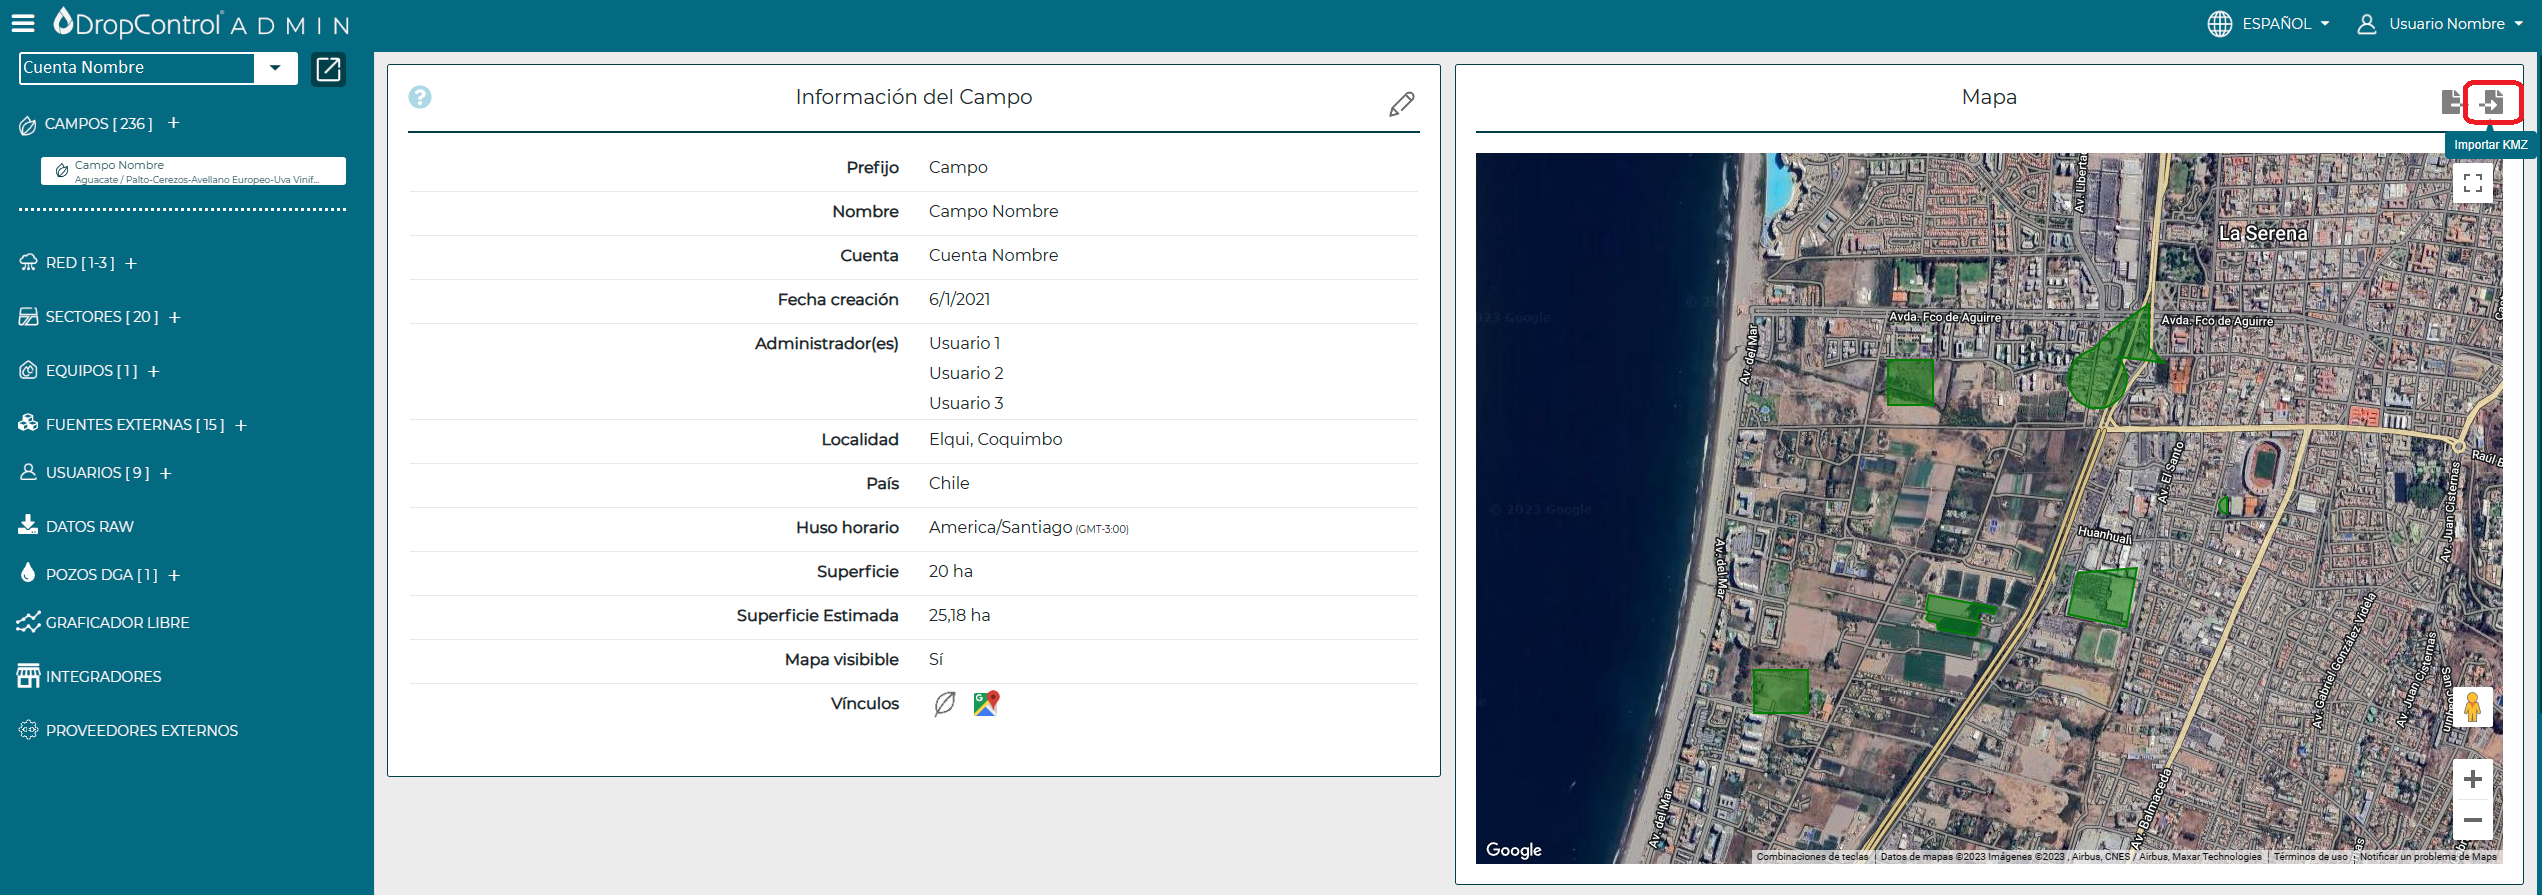
\includegraphics[width=0.8\textwidth]{mapcfg-1}
	\caption{\label{fig:mapcfg-1} Como ingresar al configurador de mapa}
\end{figure}

Al ingresar a esta herramienta, el usuario se encontrará con 2 secciones como se muestra en la figura \ref{fig:mapcfg-2}, teniendo a la izquierda la tabla de sectores y nodos y a la derecha el mapa.

\begin{figure}[H]
	\centering
	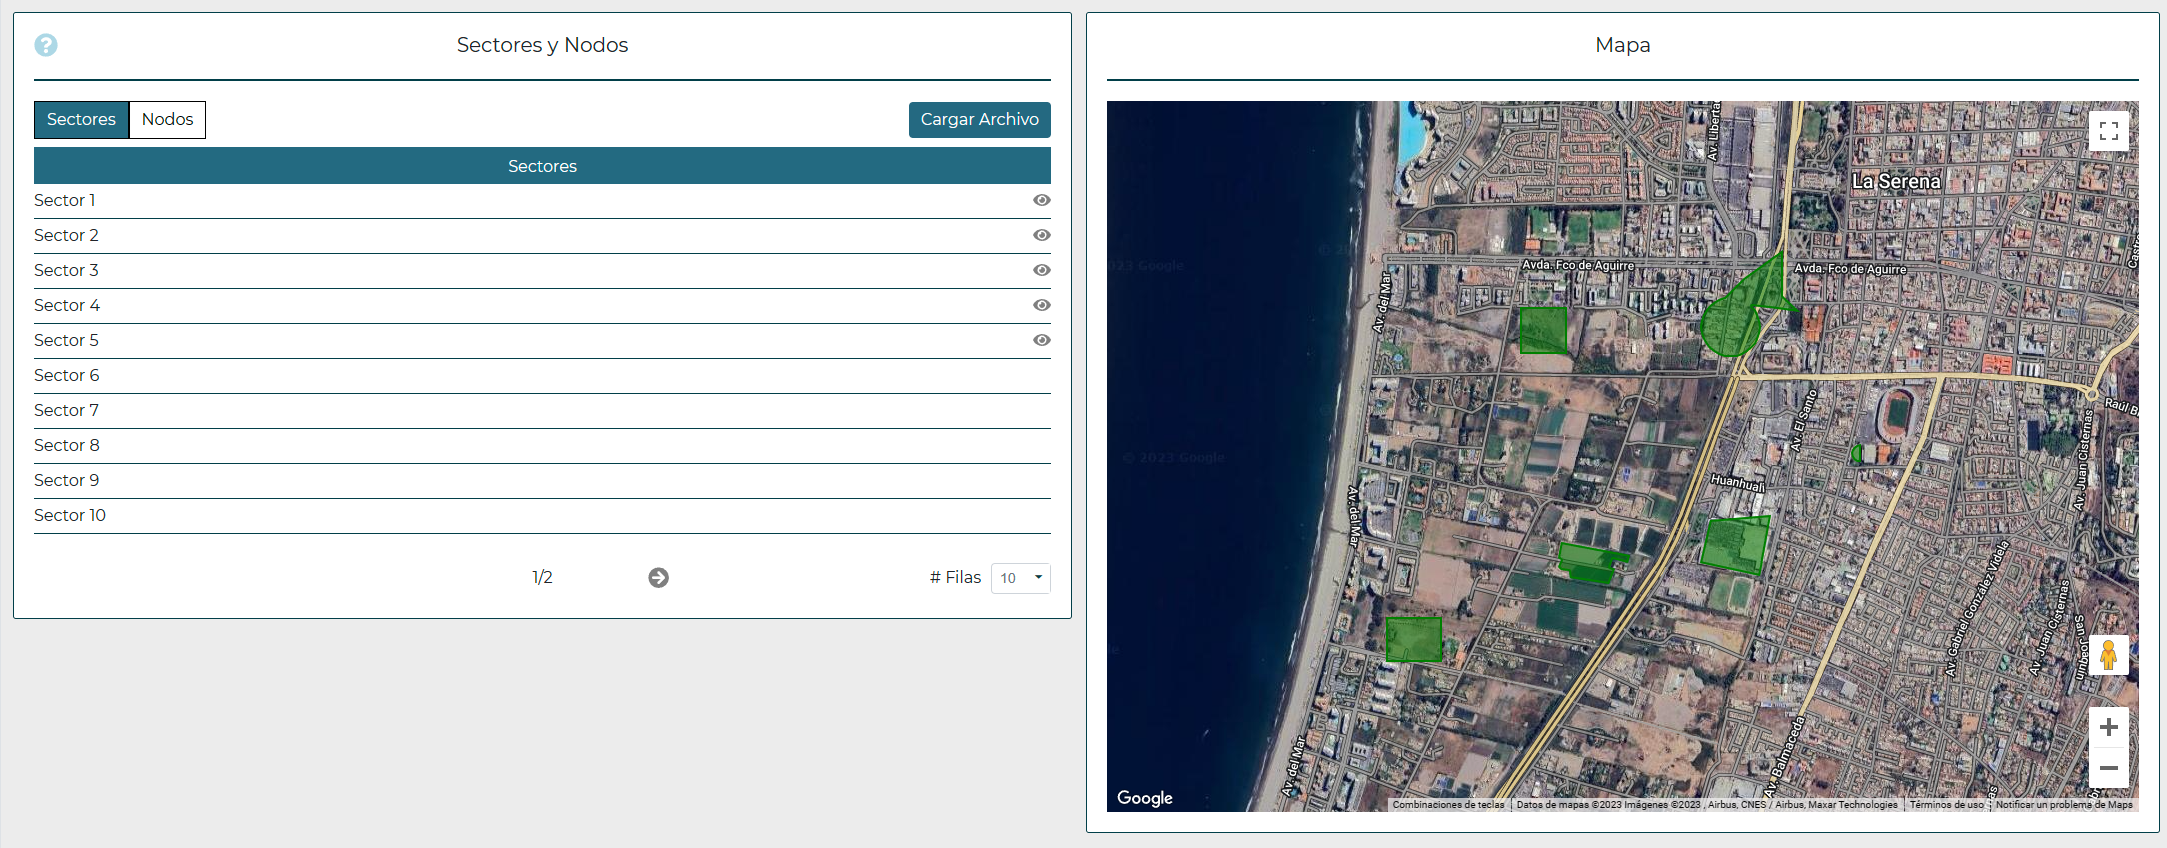
\includegraphics[width=0.8\textwidth]{mapcfg-2}
	\caption{\label{fig:mapcfg-2} Configurador de mapa}
\end{figure}

En la tabla, para cambiar entre sectores y nodos se debe hacer click en los botones de la esquina superior izquierda de la tabla.

\begin{figure}[H]
	\centering
	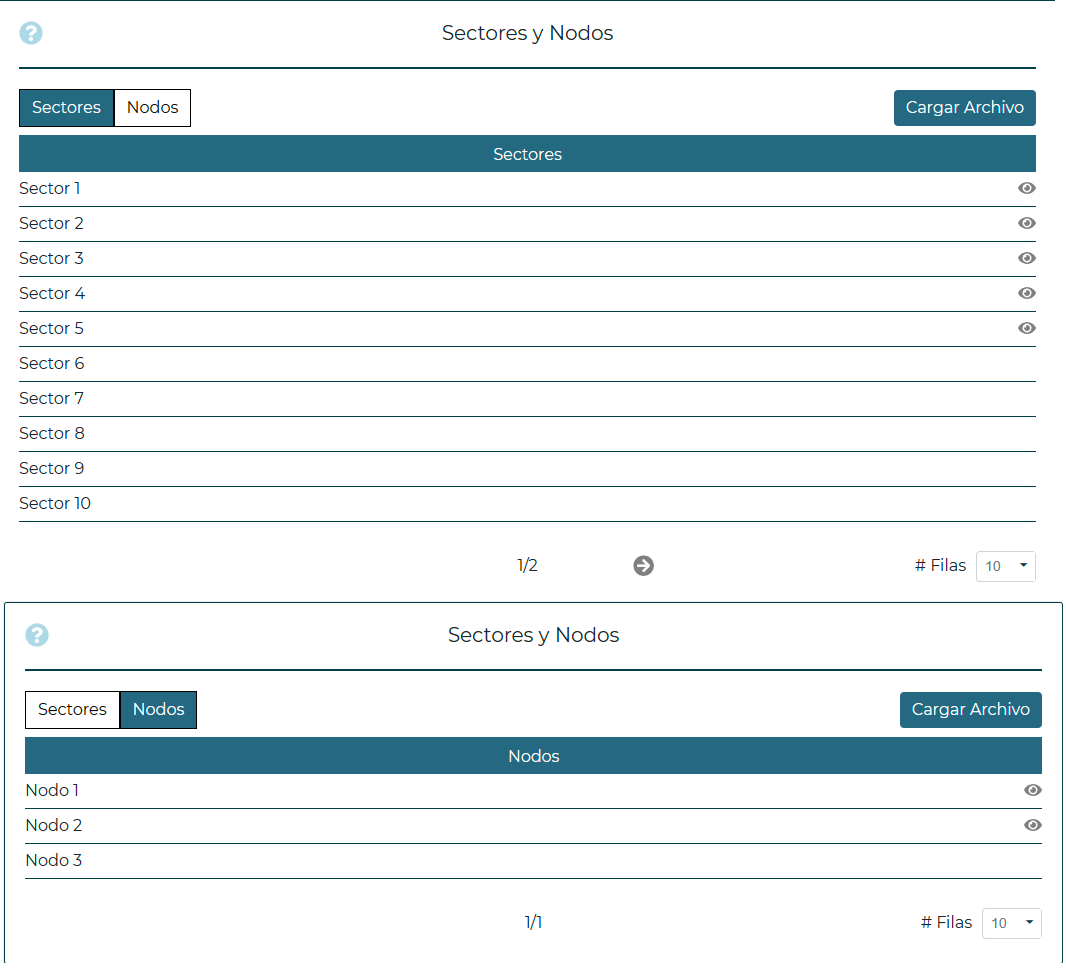
\includegraphics[width=0.8\textwidth]{mapcfg-tables}
	\caption{\label{fig:mapcfg-tables} Tabla de nodos y sectores}
\end{figure}

El mapa mostrará sectores o nodos según la tabla seleccionada como se ve en la figura \ref{fig:mapcfg-maps}. El primer mapa muestra los sectores representados por polígonos, mientras que, el segundo mapa muestra los nodos representados por marcadores. Como muestra en la figura, los sectores ya asignados son polígonos verdes y los nodos tienen un ícono según su tipo.

\begin{figure}[H]
	\centering
	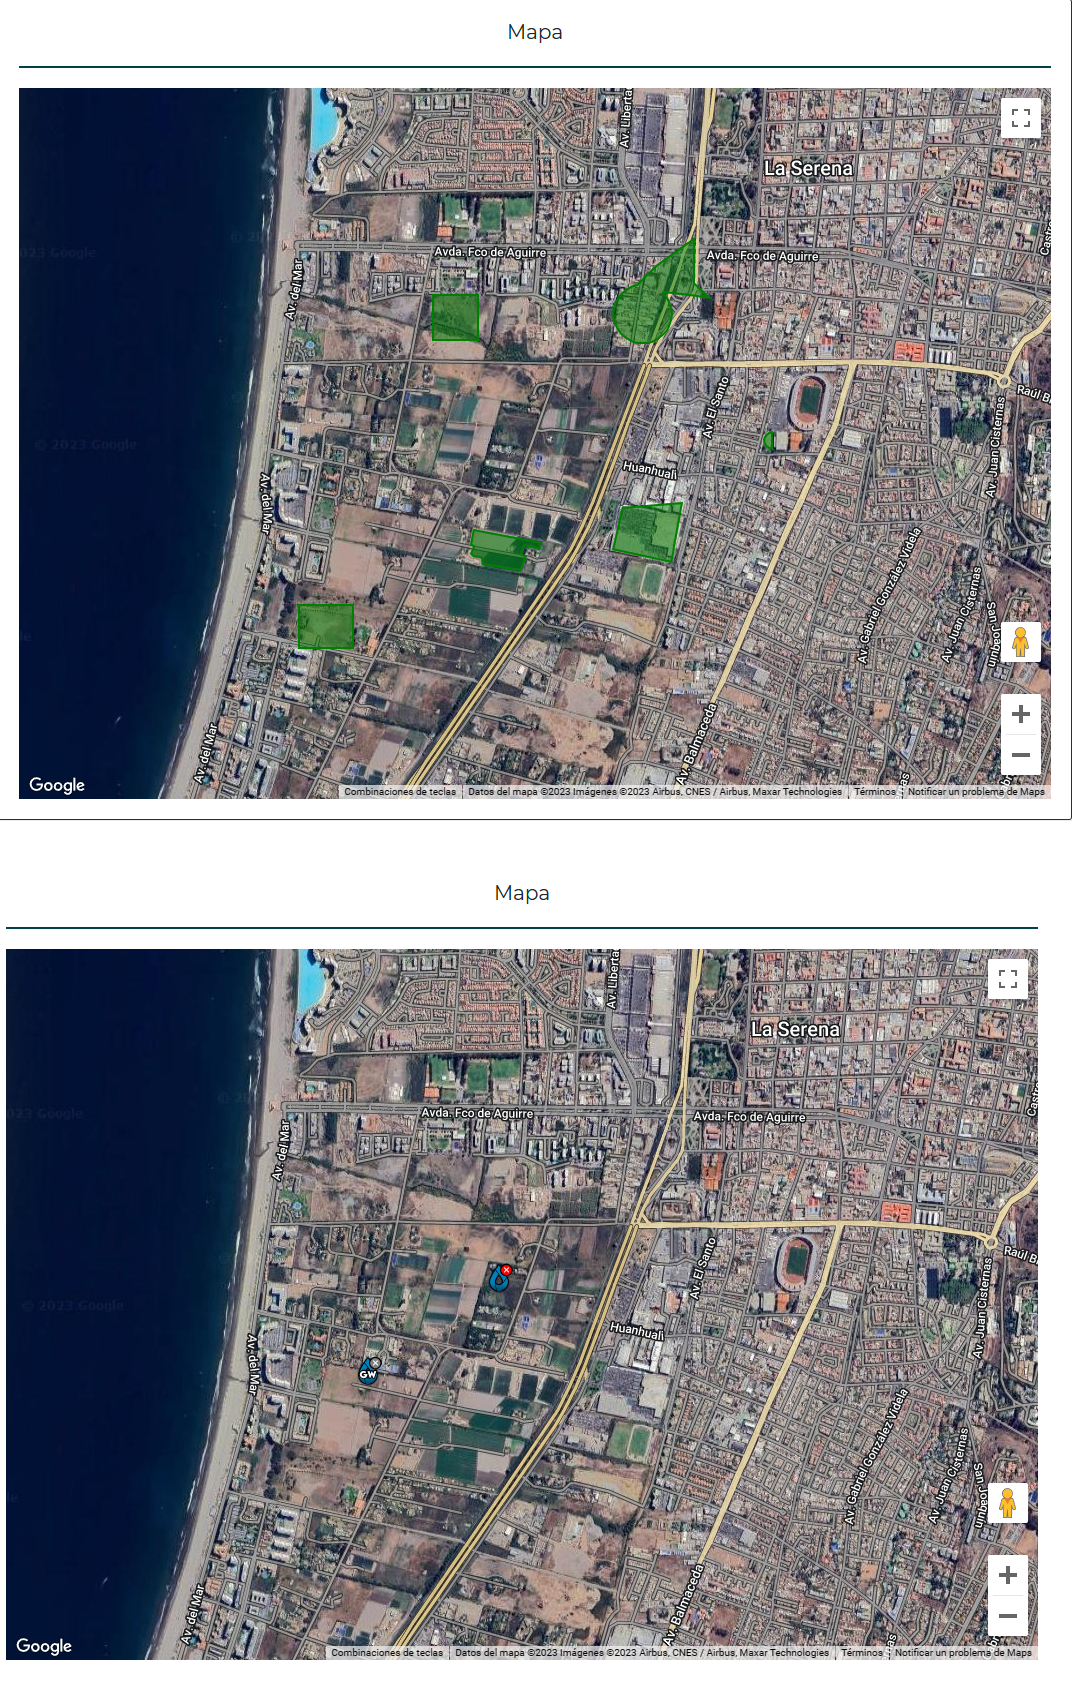
\includegraphics[width=0.8\textwidth]{mapcfg-maps}
	\caption{\label{fig:mapcfg-maps} Tabla de nodos y sectores}
\end{figure}

Para cargar el archivo que contiene nuestros sectores y/o nodos, se debe hacer click sobre el botón de 'Cargar Archivo', como se muestra en la figura \ref{fig:mapcfg-load-file}

\begin{figure}[H]
	\centering
	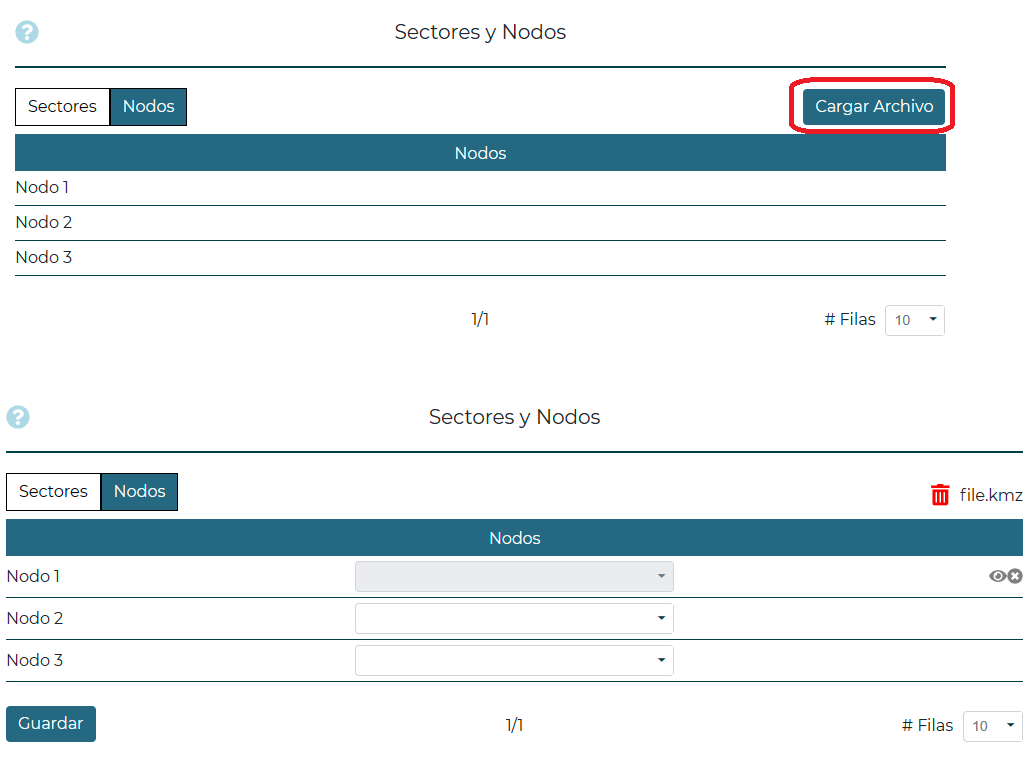
\includegraphics[width=0.8\textwidth]{mapcfg-load-file}
	\caption{\label{fig:mapcfg-load-file} Carga de archivo .kmz}
\end{figure}

Al cargar el archivo .kmz, en las tablas se agrega una columna en medio con un selector como se aprecia en la figura \ref{fig:mapcfg-tables-edit}

\begin{figure}[H]
	\centering
	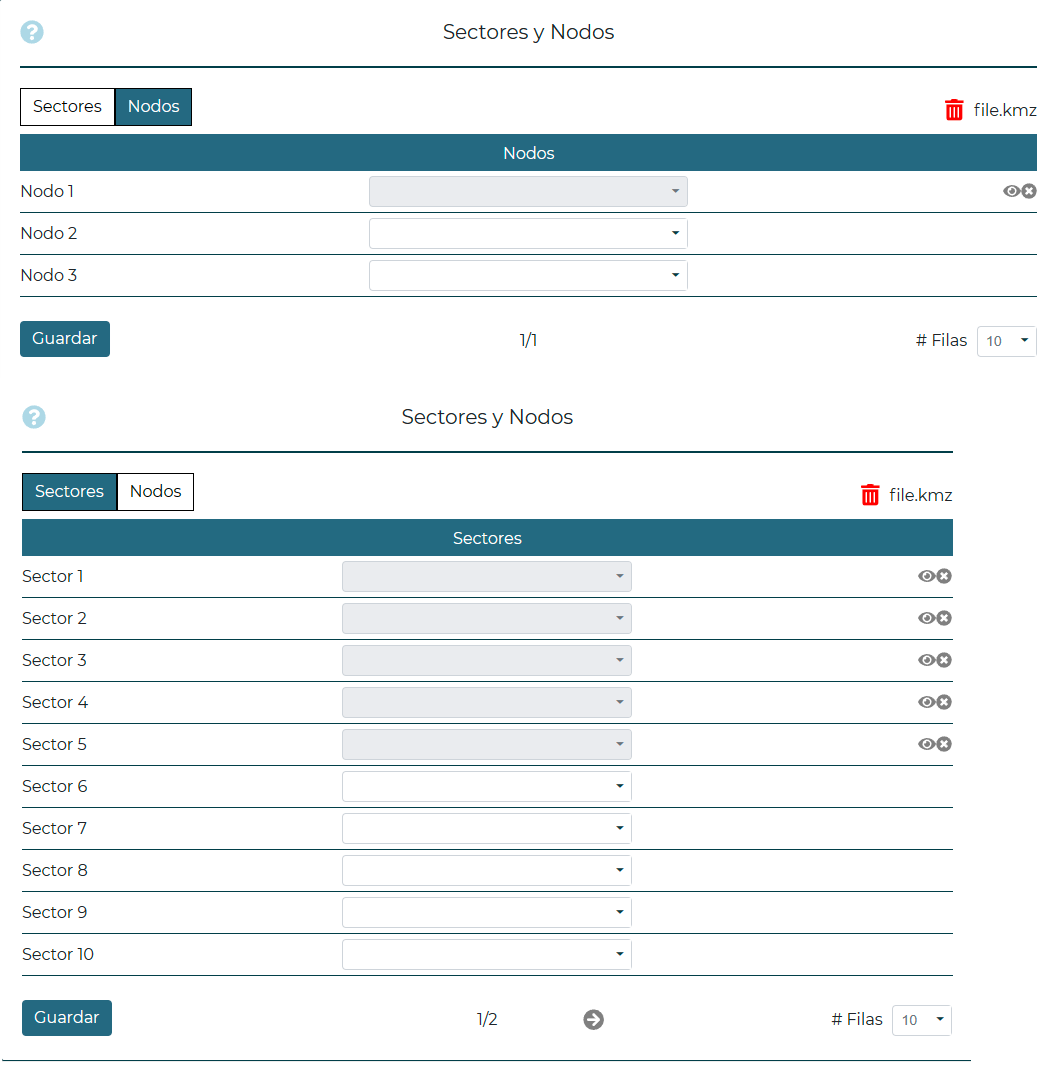
\includegraphics[width=0.8\textwidth]{mapcfg-tables-edit}
	\caption{\label{fig:mapcfg-tables-edit} Tablas de sectores y nodos al cargar un archivo.}
\end{figure}

En el mapa se agregan los polígonos del archivo con un color celeste (figura \ref{fig:mapcfg-cfg-map-zone}), mientras que los marcadores se muestran con un punto con un borde negro y centro azul (figura \ref{fig:mapcfg-cfg-map-node}).

\begin{figure}[H]
	\centering
	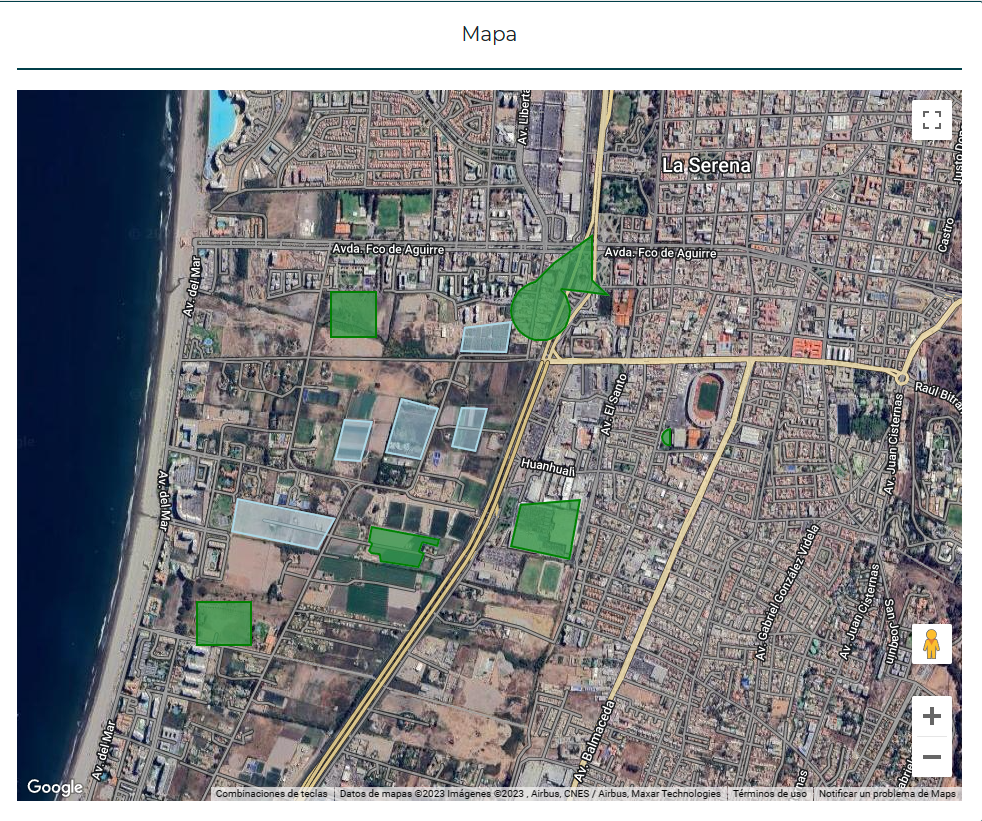
\includegraphics[width=0.8\textwidth]{mapcfg-cfg-map-zone}
	\caption{\label{fig:mapcfg-cfg-map-zone} Tablas de sectores y nodos al cargar un archivo.}
\end{figure}

\begin{figure}[H]
	\centering
	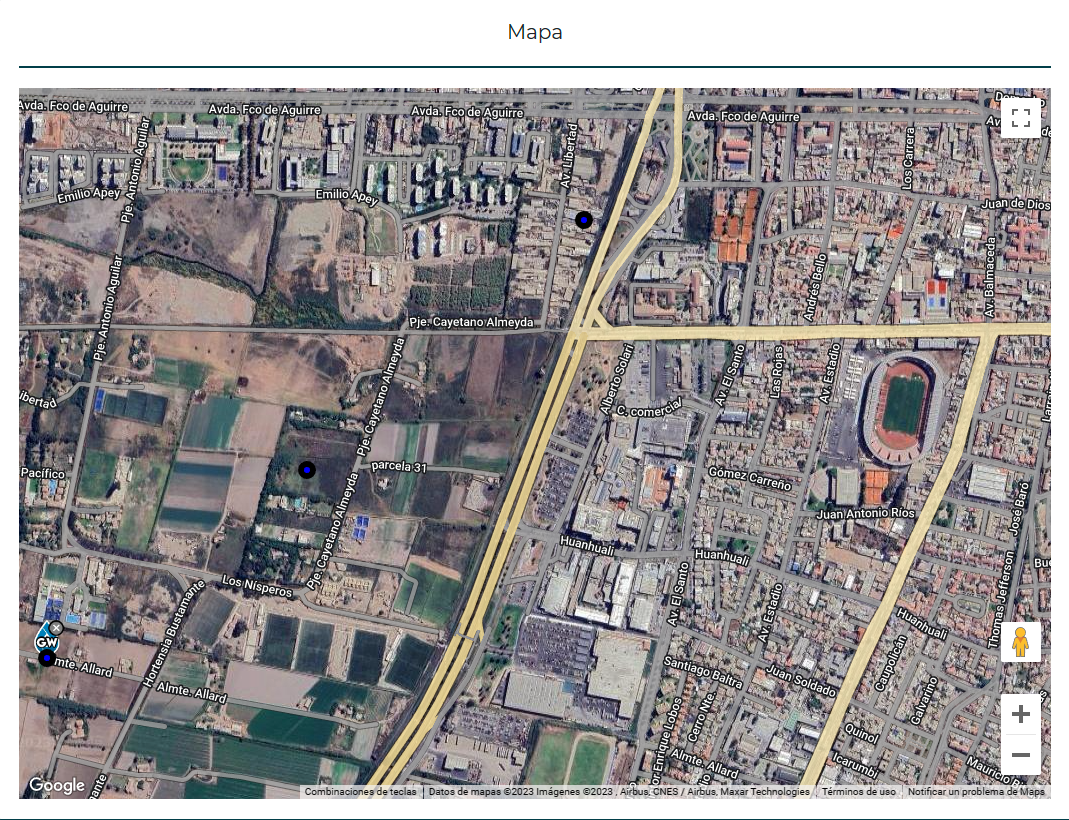
\includegraphics[width=0.8\textwidth]{mapcfg-cfg-map-node}
	\caption{\label{fig:mapcfg-cfg-map-node} Tablas de sectores y nodos al cargar un archivo.}
\end{figure}

\subsubsubsection{DATOS}

En el año 2023, como muestra la figura \ref{fig:mapcfg-analytics-view} el configurador de mapa tuvo 769 vistas, con un total de 187 usuarios y con una retención de aproximadamente 3 minutos.
\begin{figure}[H]
	\centering
	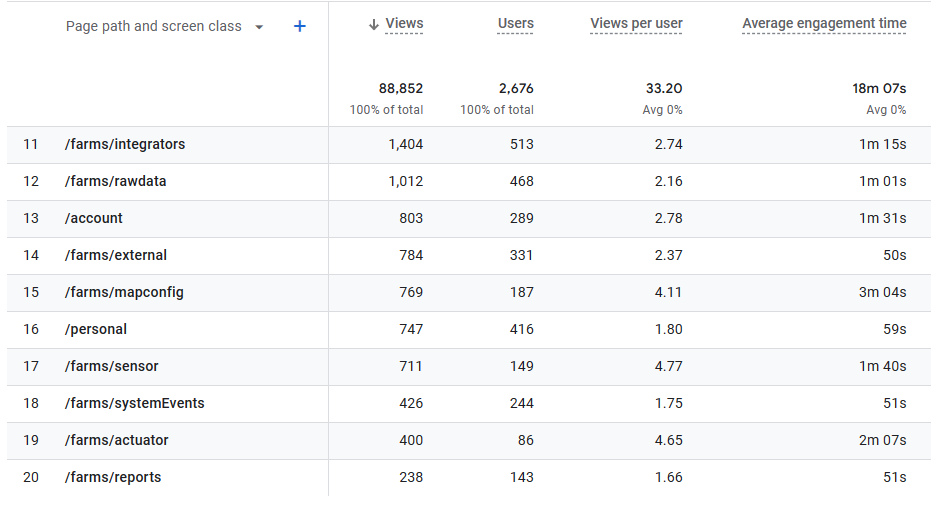
\includegraphics[width=0.8\textwidth]{mapcfg-analytics-view}
	\caption{\label{fig:mapcfg-analytics-view} Datos de vistas de la herramienta de configurador de mapa en el año 2023.}
\end{figure}
\iffalse
\subsubsection{GRAFICADOR LIBRE}

\subsubsubsection{FUNCIONAMIENTO}

Esta nueva herramienta implementada en la aplicación de \textit{Admin de DropControl} se encuentra en el menú lateral como muestra en la figura \ref{fig:menu-admin-graf}

\begin{figure}[H]
	\centering
	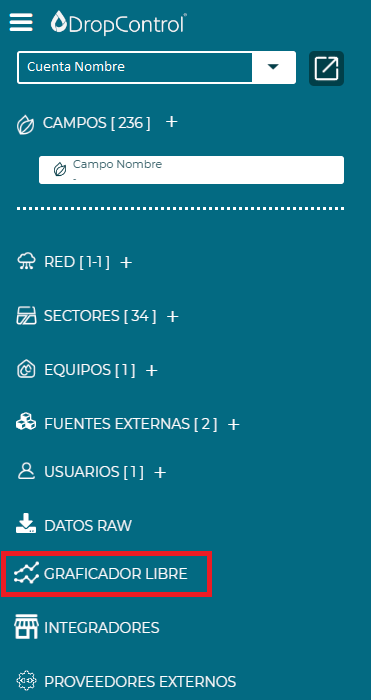
\includegraphics[width=0.5\textwidth]{menu-admin-graficador}
	\caption{\label{fig:menu-admin-graf} Graficador Libre en el menú de \textit{Admin}}
\end{figure}

En la herramienta se encontrará con 4 secciones, como se muestra en la figura \ref{fig:graf1}:
\begin{enumerate}
    \item Selección de nodo/sensores.
    \item Selección de rango de fechas.
    \item Gráfico.
    \item Tabla de datos.
\end{enumerate}

\begin{figure}[H]
	\centering
	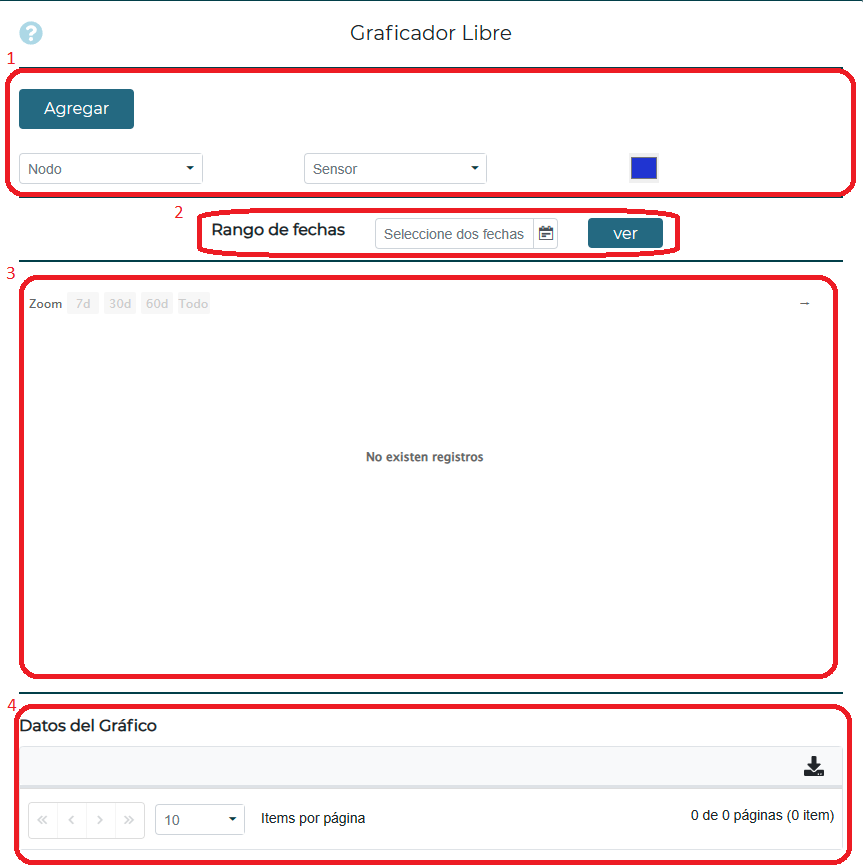
\includegraphics[width=0.8\textwidth]{graficador-1}
	\caption{\label{fig:graf1} Secciones del graficador libre}
\end{figure}

El primer paso es escoger los sensores que queremos visualizar en el gráfico, en la primera sección selecciones en el primer selector el nodo seguido del sensor y opcionalmente el color (figura \ref{fig:grafselect}).

\begin{figure}[H]
	\centering
	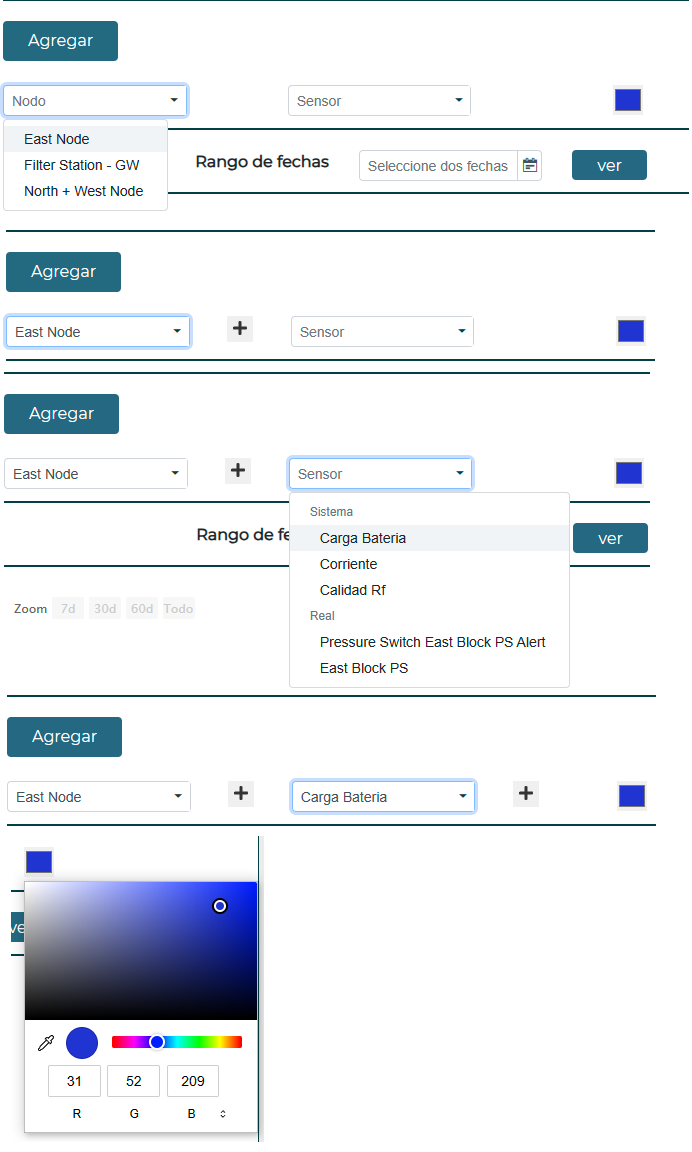
\includegraphics[width=0.8\textwidth]{graf-select}
	\caption{\label{fig:grafselect} Selección de sensor}
\end{figure}

Para escoger otro sensor se puede hacer agregando otra fila vacía haciendo click en el botón 'Agregar' (figura \ref{fig:graf-add-row-1}) y repitiendo el paso anterior.

\begin{figure}[H]
	\centering
	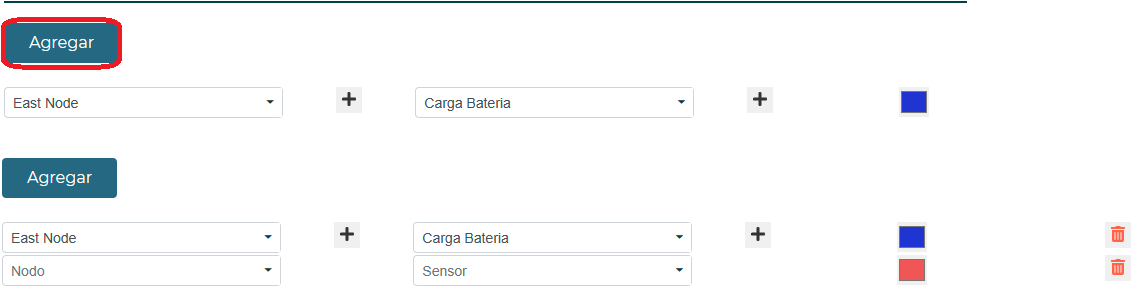
\includegraphics[width=0.8\textwidth]{graf-add-row-1}
	\caption{\label{fig:graf-add-row-1} Agregar una nueva fila vacía}
\end{figure}

Otra forma de agregar sensores es con los botones con el símbolo '+' presente en las filas. El primer botón agrega una nueva fila con el siguiente nodo seleccionado junto al sensor del mismo tipo (figura \ref{fig:graf-add-row-2}), mientras que el segundo botón agrega una nueva fila con el mismo nodo seleccionado pero con el siguiente sensor en la lista (figura \ref{fig:graf-add-row-3}).

\begin{figure}[H]
	\centering
	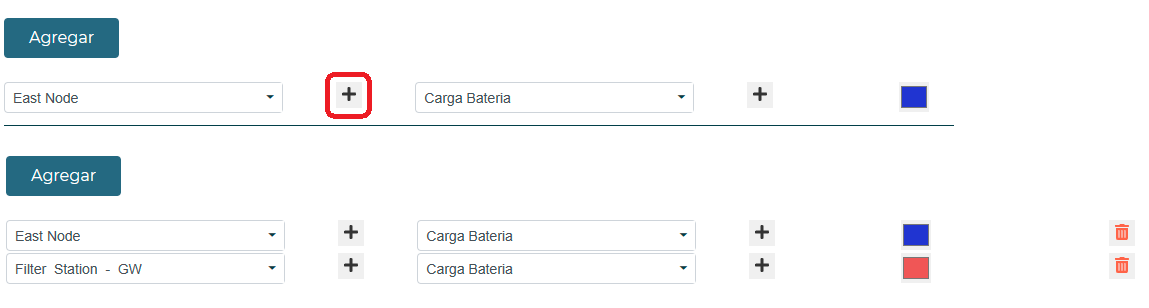
\includegraphics[width=0.8\textwidth]{graf-add-row-2}
	\caption{\label{fig:graf-add-row-2} Agregar una nueva fila con el siguiente nodo}
\end{figure}

\begin{figure}[H]
	\centering
	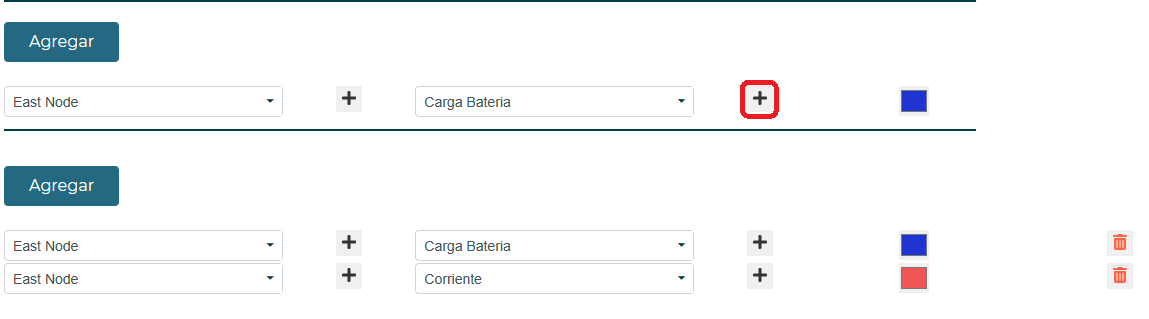
\includegraphics[width=0.8\textwidth]{graf-add-row-3}
	\caption{\label{fig:graf-add-row-3} Agregar una nueva fila con el siguiente sensor del nodo}
\end{figure}

Para eliminar una fila se debe hacer click en el último botón de la fila, con símbolo de basura (figura \ref{fig:graf-delete-row}).

\begin{figure}[H]
	\centering
	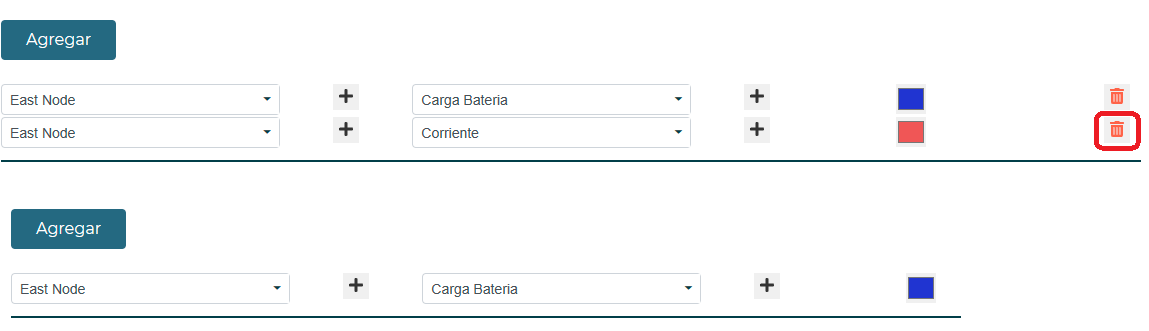
\includegraphics[width=0.8\textwidth]{graf-delete-row}
	\caption{\label{fig:graf-delete-row} Agregar una nueva fila con el siguiente sensor del nodo}
\end{figure}

El siguiente paso es escoger el rango de fechas de los datos, como se muestra en la figura \ref{fig:graf-date-range-1}.

\begin{figure}[H]
	\centering
	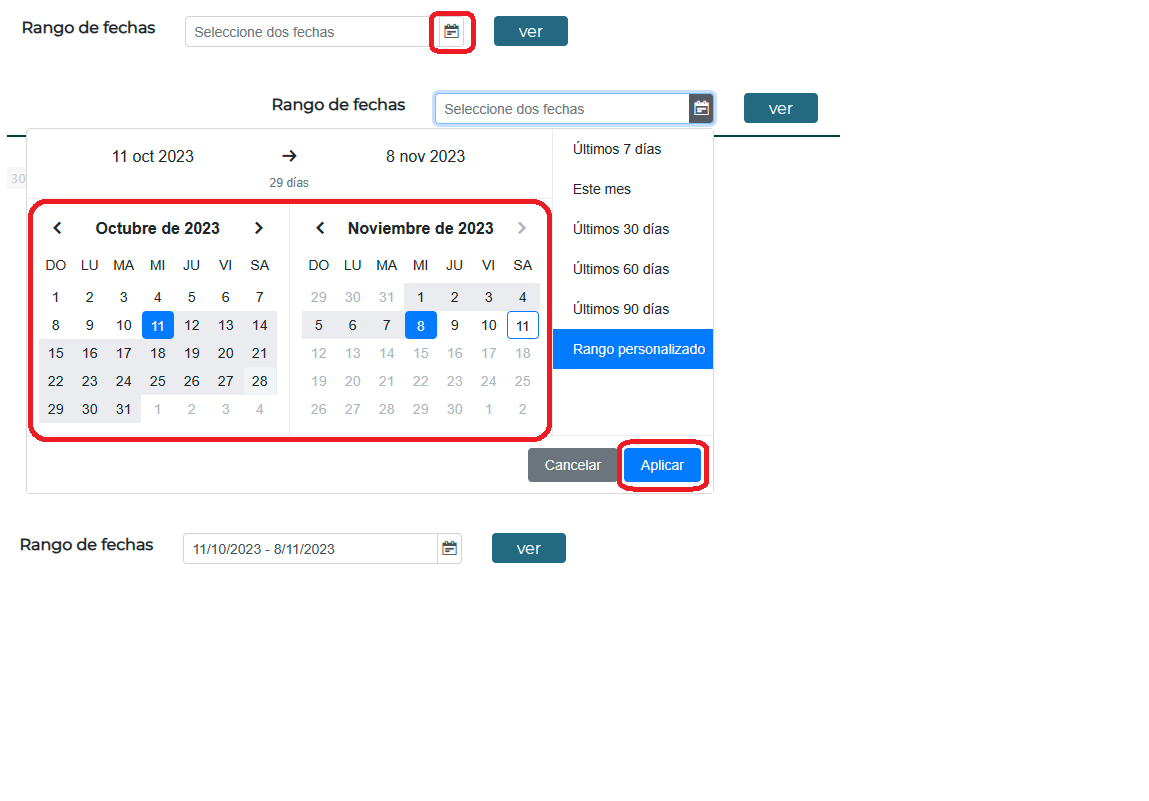
\includegraphics[width=0.8\textwidth]{graf-date-range-1}
	\caption{\label{fig:graf-date-range-1} Selección de rango de fechas}
\end{figure}

Se puede escoger un rango personalizado, como se mostró anteriormente, o escoger rangos predeterminados como muestra en la figura \ref{fig:graf-date-range-2}.

\begin{figure}[H]
	\centering
	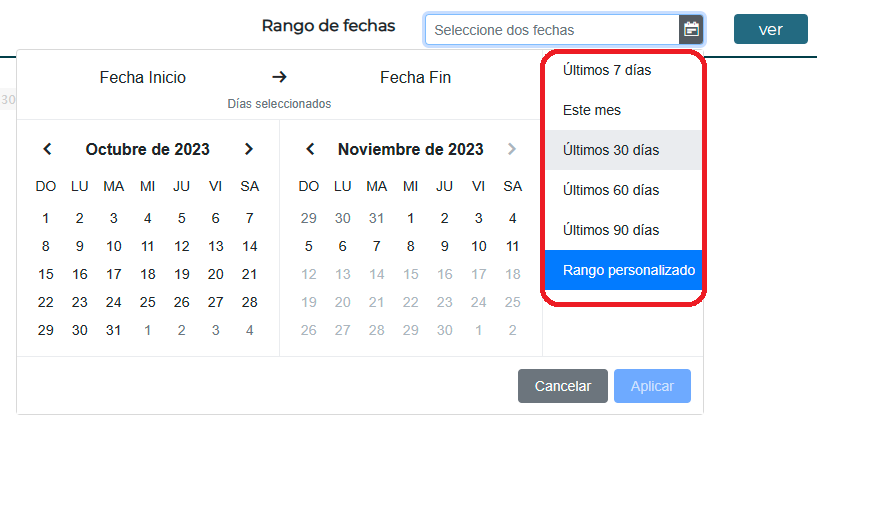
\includegraphics[width=0.8\textwidth]{graf-date-range-2}
	\caption{\label{fig:graf-date-range-2} Selección de rango de fechas}
\end{figure}

Luego de tener el rango de fechas seleccionado, hacer click en el botón 'ver' para mostrar los datos de los sensores seleccionados (figura \ref{fig:graf-display-1})

\begin{figure}[H]
	\centering
	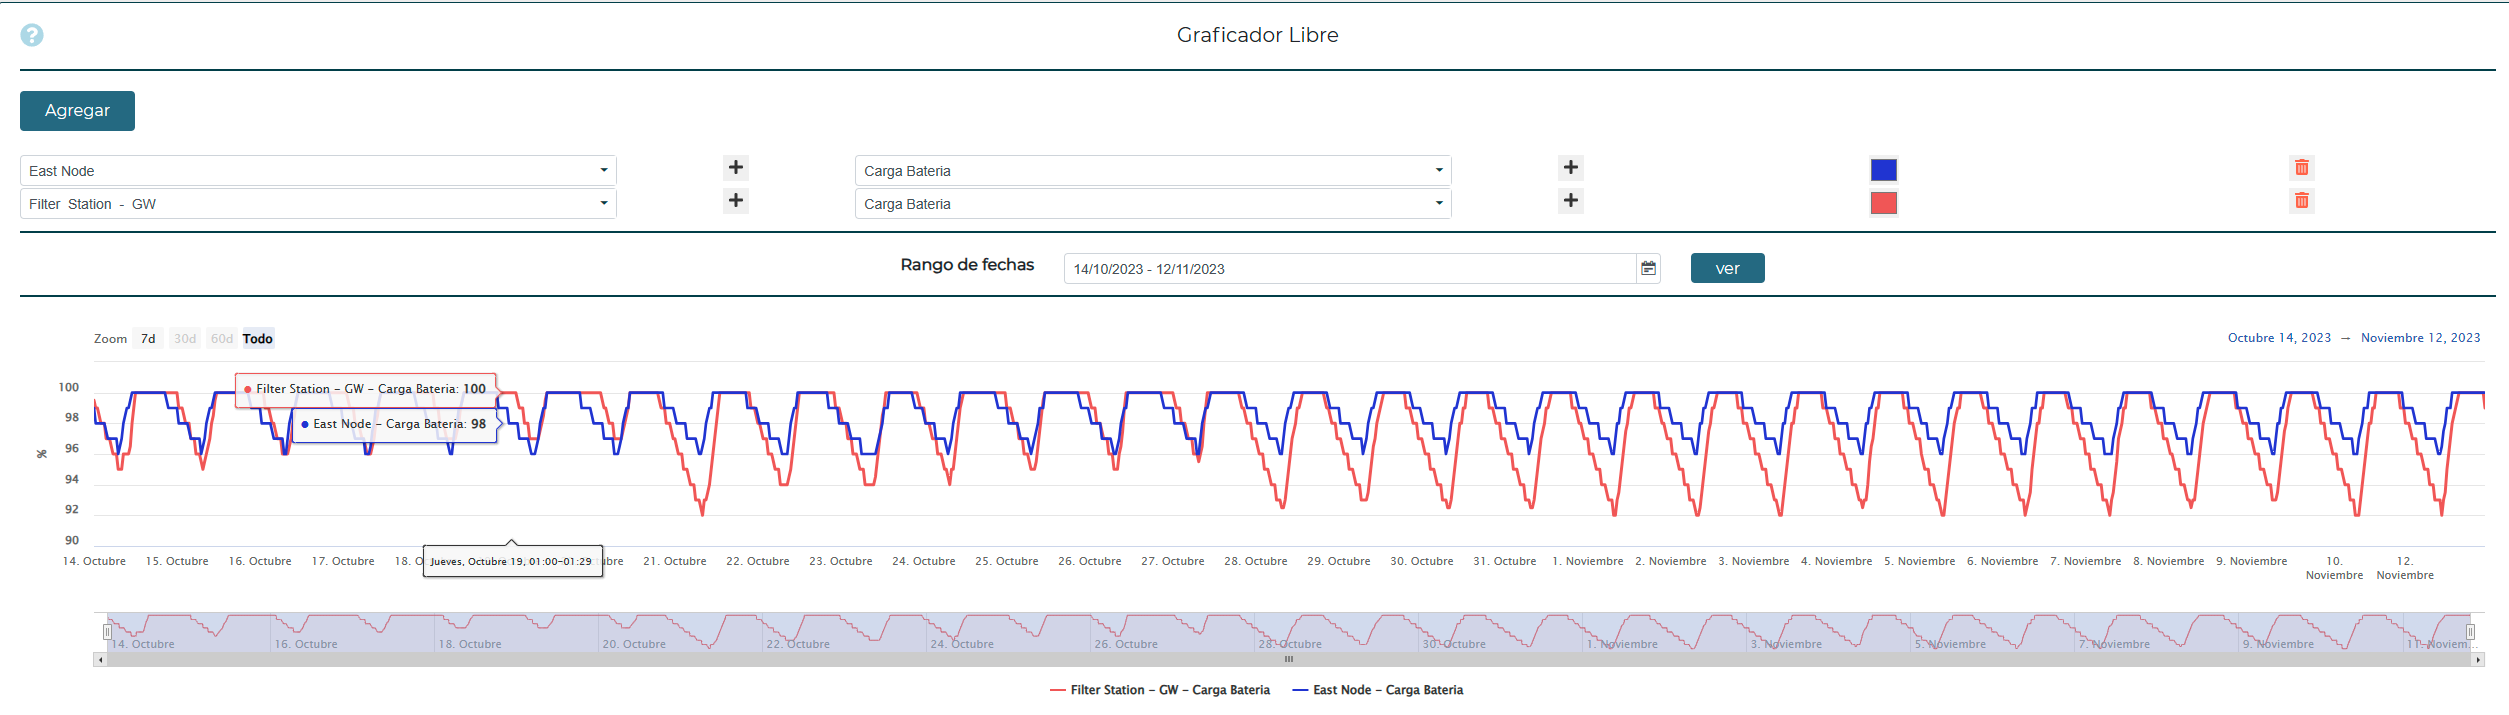
\includegraphics[width=0.8\textwidth]{graf-display-1}
	\caption{\label{fig:graf-display-1} Gráfico}
\end{figure}

En la última sección se encuentra la tabla de datos del gráfico, en donde se muestran los datos de los sensores donde la primera columna es la fecha y hora del dato y las columnas siguientes son los sensores escogidos con el formato de nombre \{Nodo\}-\{Sensor\} [unidad] (figura \ref{fig:graf-table-1}). 
Además, tiene la funcionalidad de exportar la tabla en formato .xlsx haciendo click en el ícono de descarga en la esquina superior derecha de la tabla.

\begin{figure}[H]
	\centering
	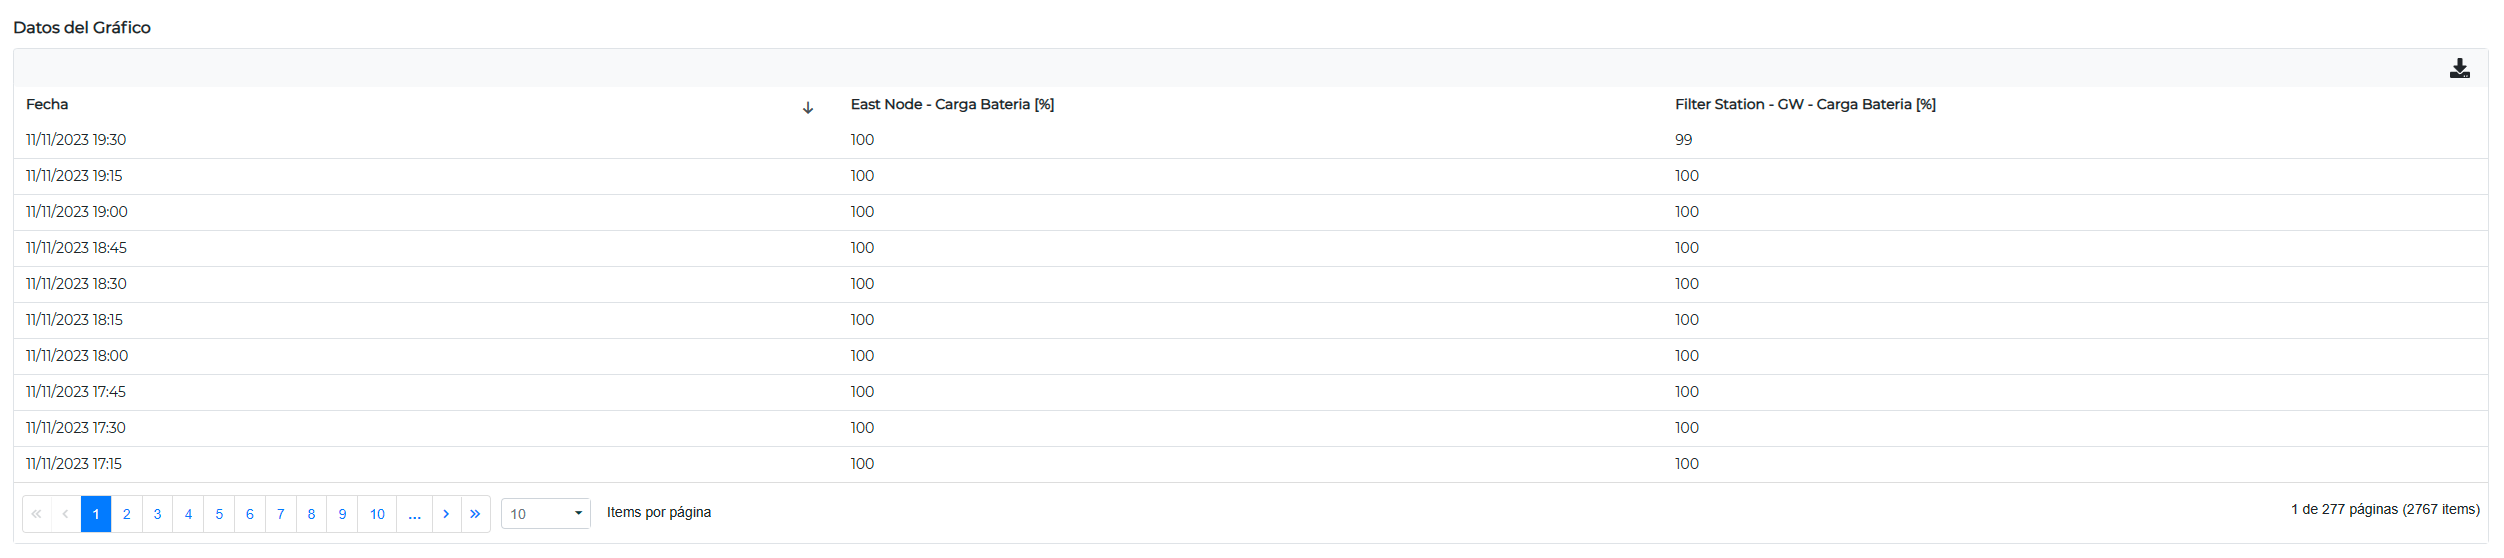
\includegraphics[width=0.8\textwidth]{graf-table-1}
	\caption{\label{fig:graf-table-1} Gráfico}
\end{figure}


\subsubsection{DATOS}

En el año 2023, como muestra la figura \ref{fig:graf-analytics-view} el configurador de mapa tuvo 2947 vistas, con un total de 533 usuarios y con una retención de aproximadamente 1 minuto.
\begin{figure}[H]
	\centering
	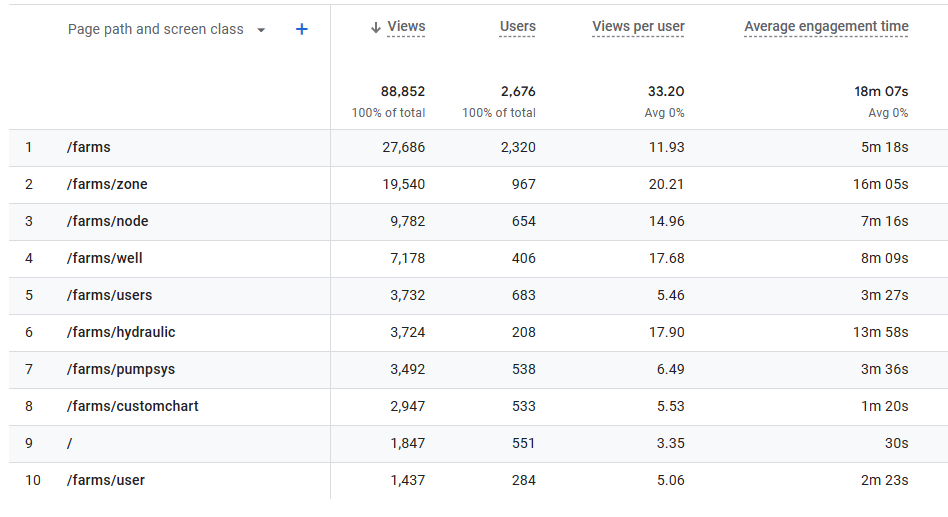
\includegraphics[width=0.8\textwidth]{graf-analytics-view}
	\caption{\label{fig:graf-analytics-view} Datos de vistas de la herramienta de graficador libre en el año 2023.}
\end{figure}
\fi

\subsection{OPERATIONS}

\subsubsection{DESPACHOS MÚLTIPLES}

Entrando a la herramienta de \textit{Operations}, en el menú lateral, abrir la sección de Despachos y se encuentran las opciones de 'Individuales' y 'Múltiples' (Figura \ref{fig:op-menu}).

\begin{figure}[H]
	\centering
	\includegraphics[width=1\textwidth]{validation-op-dm/menu.png}
	\caption{\label{fig:op-menu} Menu de Despachos en \textit{Operations}}
\end{figure}

Al hacer click en 'Múltiples' se ingresa a la sección de despachos múltiples (Figura \ref{fig:op-list}).
Se tiene una tabla con los despachos múltiples creados.

\begin{figure}[H]
	\centering
	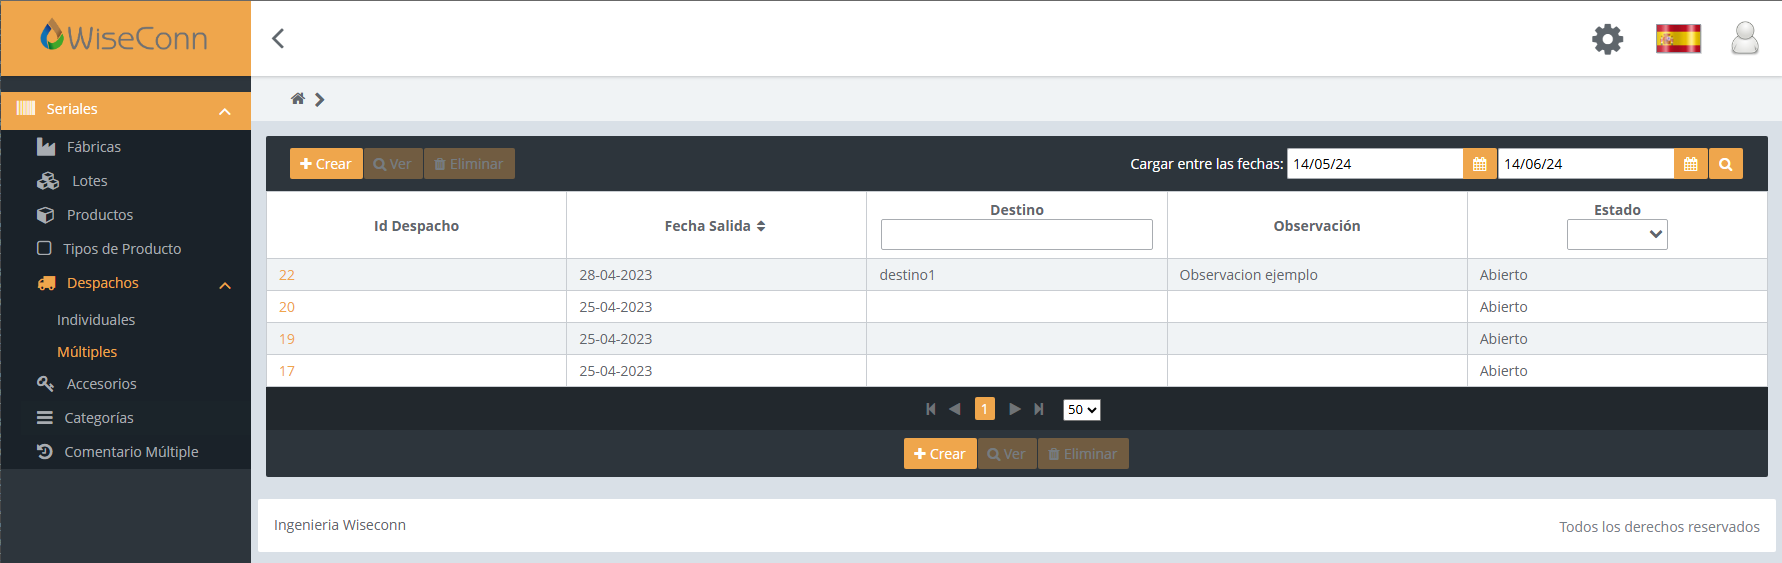
\includegraphics[width=0.8\textwidth]{validation-op-dm/list.png}
	\caption{\label{fig:op-list} Menu de Despachos en \textit{Operations}}
\end{figure}

Para crear un despacho múltiple se debe hacer click en el botón 'Crear' en la tabla. Al hacer click, se abrirá el formulario de la figura \ref{fig:op-form-create-1}.
Los parámetros previos al 'Número de despachos' son los parámetros del despacho padre, el cual los despachos hijos herederan.

\begin{figure}[H]
	\centering
	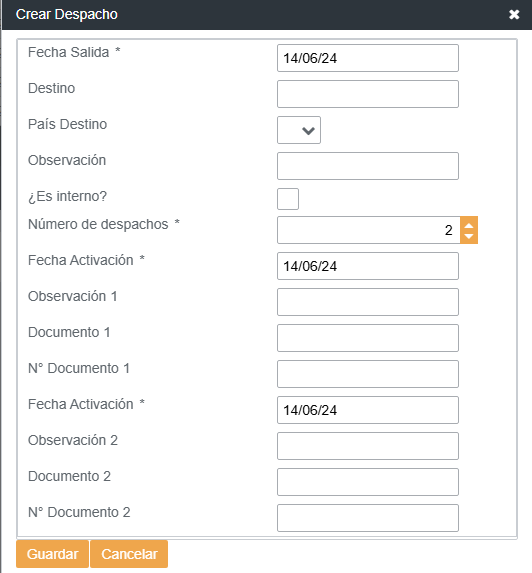
\includegraphics[width=1\textwidth]{validation-op-dm/form-create-1.png}
	\caption{\label{fig:op-form-create-1} Formulario de creación de Despacho Múltiple}
\end{figure}

El parámetros 'Número de despachos' indica, valga la redundancia, el número de despachos hijos. Esto se aprecia al comparar la figura \ref{fig:op-form-create-1} y la figura \ref{fig:op-form-create-2}.

\begin{figure}[H]
	\centering
	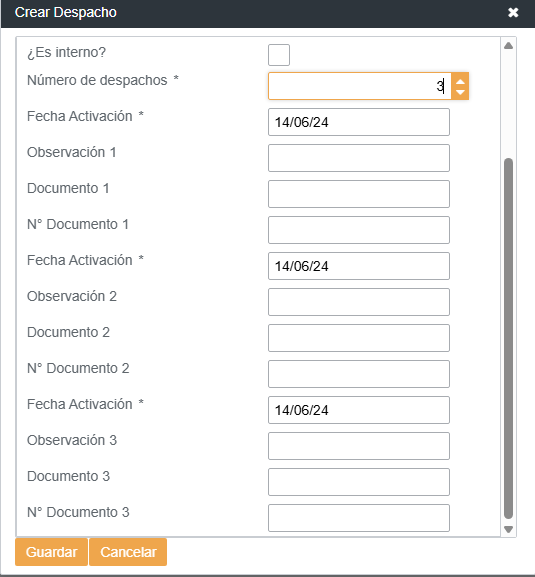
\includegraphics[width=1\textwidth]{validation-op-dm/form-create-2.png}
	\caption{\label{fig:op-form-create-2} Formulario de creación de Despacho Múltiple con 3 despachos}
\end{figure}

\subsubsection{ACTUALIZACIÓN MASIVA DE PRODUCTOS}

En el menú lateral, la funcionalidad se encuentra bajo el nombre de 'Comentario múltiple' (figura \ref{fig:op-menu-cm}).

\begin{figure}[H]
	\centering
	\includegraphics[width=1\textwidth]{validation-op-cm/menu.png}
	\caption{\label{fig:op-menu-cm} Comentario Múltiple en menú}
\end{figure}

Al ingresar a la funcionalidad, en la sección izquierda se encuentra formulario para ingresar el comentario, mientras que, en la sección derecha se encuentra la tabla de productos al que se le asignará el comentario (figura \ref{fig:op-view-cm}).

\begin{figure}[H]
	\centering
	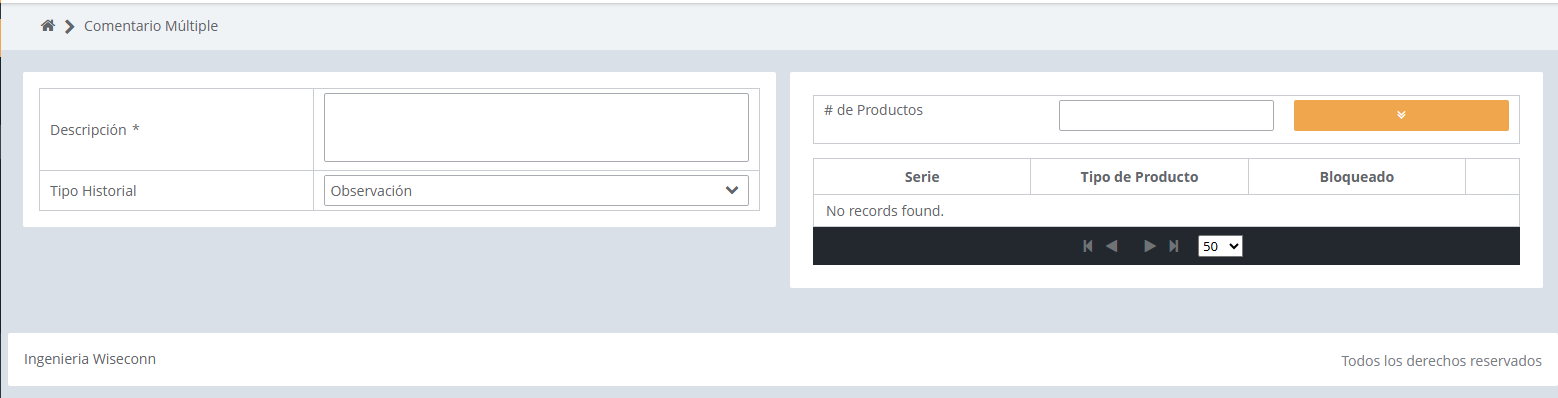
\includegraphics[width=1\textwidth]{validation-op-cm/view.png}
	\caption{\label{fig:op-view-cm} Comentario Múltiple}
\end{figure}

En la tabla de productos se ingresan las series de productos a los cuales se quiere registrar una historia (figura \ref{fig:op-add-product-cm}).

\begin{figure}[H]
	\centering
	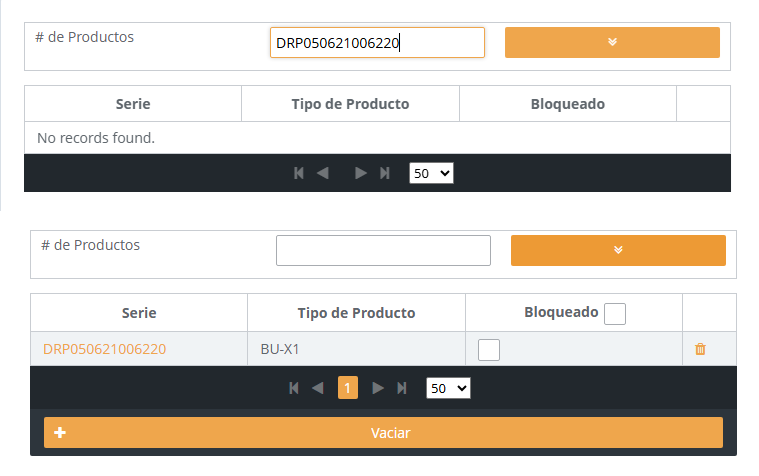
\includegraphics[width=1\textwidth]{validation-op-cm/add-product.png}
	\caption{\label{fig:op-add-product-cm} Comentario Múltiple: Agregar productos}
\end{figure}

En el formulario, si se selecciona el tipo de historial 'Fallo PreProducción' o 'Fallo PostProducción' se muestra un nuevo selector para ingresar el tipo de falla (figura \ref{fig:op-select-history-type-cm}). Estos tipos de historia también afecta la tabla de productos, agregando una nueva columna de tipo \textit{checkbox} para indicar si el producto esta reparado o no (figura \ref{fig:op-tabla-productos-reparado-col-cm}).

\begin{figure}[H]
	\centering
	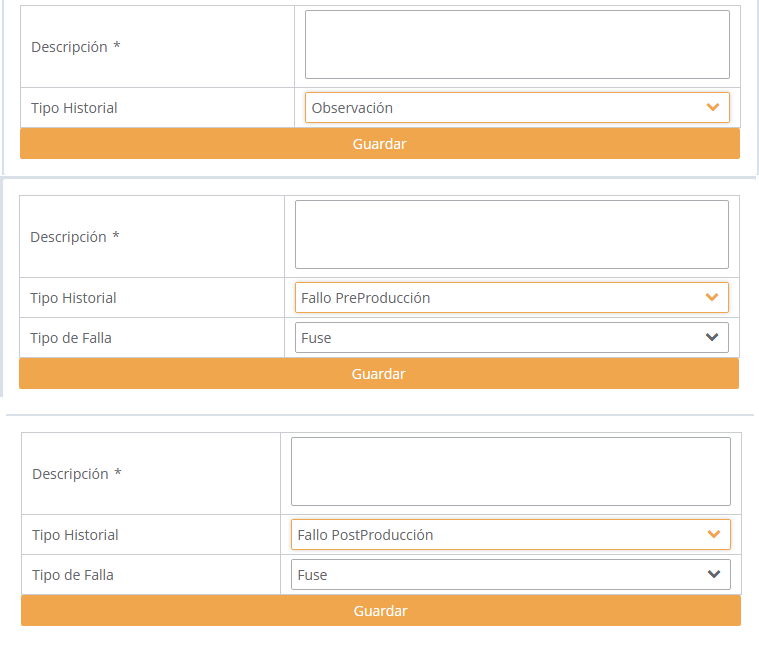
\includegraphics[width=1\textwidth]{validation-op-cm/select-history-type.png}
	\caption{\label{fig:op-select-history-type-cm} Comentario Múltiple: Tipos de historia}
\end{figure}

\begin{figure}[H]
	\centering
	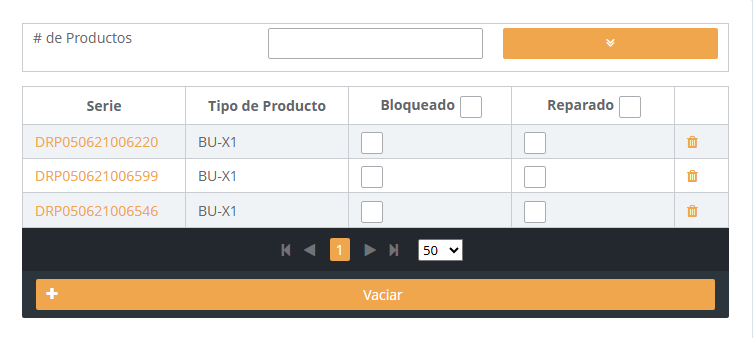
\includegraphics[width=1\textwidth]{validation-op-cm/tabla-productos-reparado-col.png}
	\caption{\label{fig:op-tabla-productos-reparado-col-cm} Comentario Múltiple: Tabla productos - Columna reparado}
\end{figure}

En la figura \ref{fig:op-test-1-cm} se ve el formulario completo. Al hacer click en guardar se mostrará un diálogo de confirmación (figura \ref{fig:op-test-1-confirm-cm}). Cuando se confirmen los cambios, se agregarán las historias a los productos correspondientes y se muestra un \textit{toast} que confirma el guardado (figura \ref{fig:op-test-1-finish-cm}).

\begin{figure}[H]
	\centering
	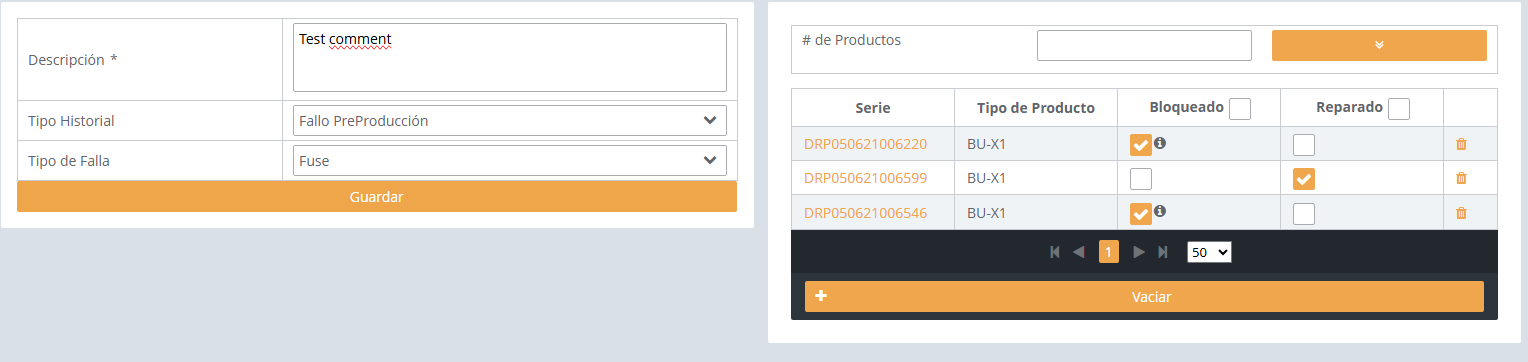
\includegraphics[width=1\textwidth]{validation-op-cm/test-1.png}
	\caption{\label{fig:op-test-1-cm} Comentario Múltiple: Formulario completo.}
\end{figure}

\begin{figure}[H]
	\centering
	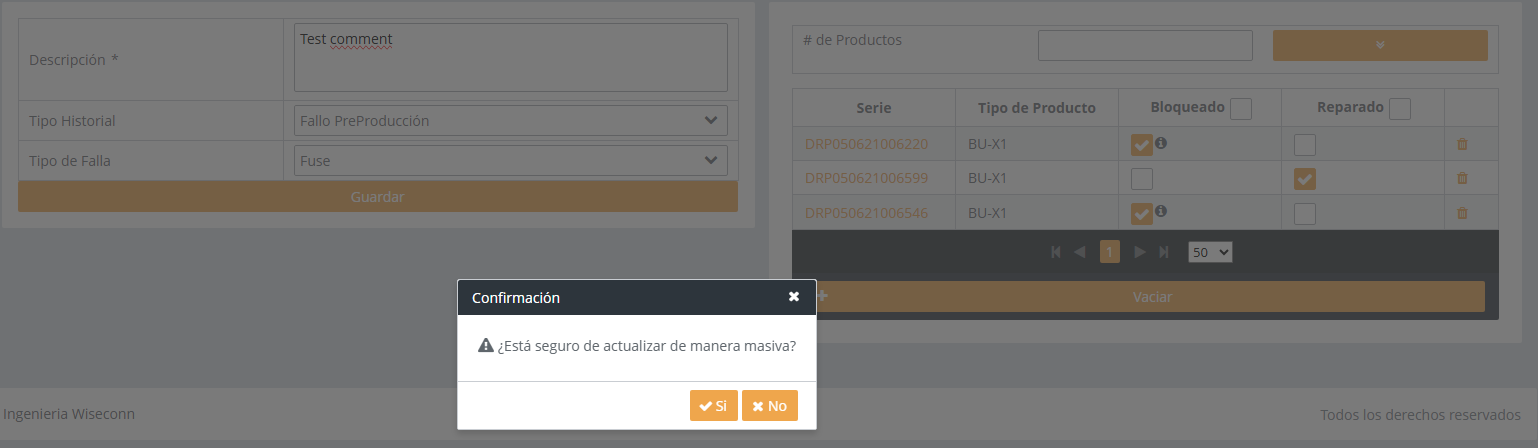
\includegraphics[width=1\textwidth]{validation-op-cm/test-1-confirm.png}
	\caption{\label{fig:op-test-1-confirm-cm} Comentario Múltiple: Confirmar cambios.}
\end{figure}

\begin{figure}[H]
	\centering
	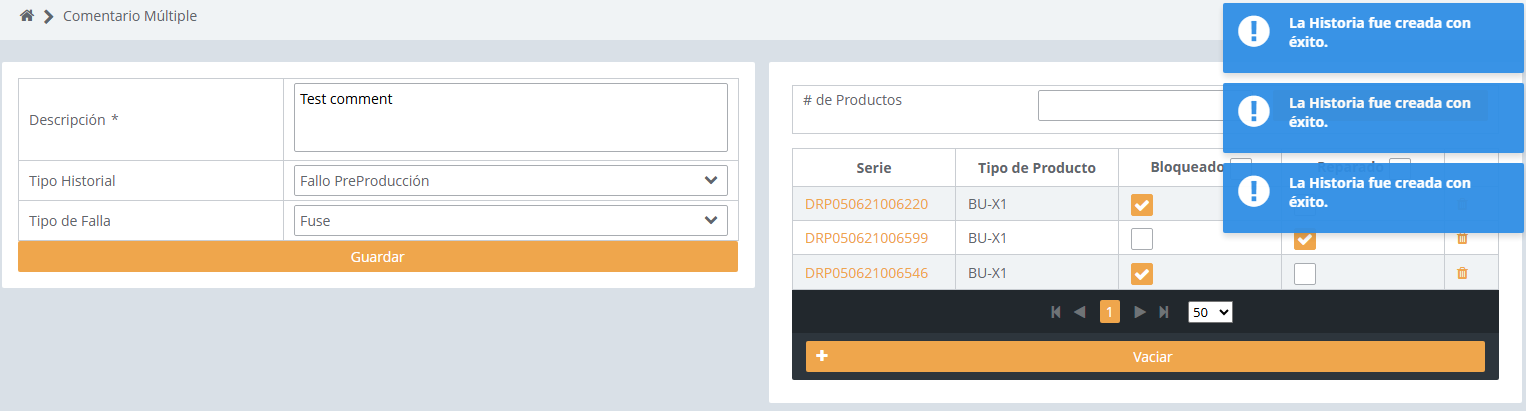
\includegraphics[width=1\textwidth]{validation-op-cm/test-1-finish.png}
	\caption{\label{fig:op-test-1-finish-cm} Comentario Múltiple: Historias registradas.}
\end{figure}

Los cambios reflejados en los productos se muestra en la figura \ref{fig:op-test-1-products-cm}, en la tabla de historias se encuentra la historia que se agregó, junto a si se marcó como reparada o no, y en la información del producto si este se marcó como bloqueado.

\begin{figure}[H]
	\centering
	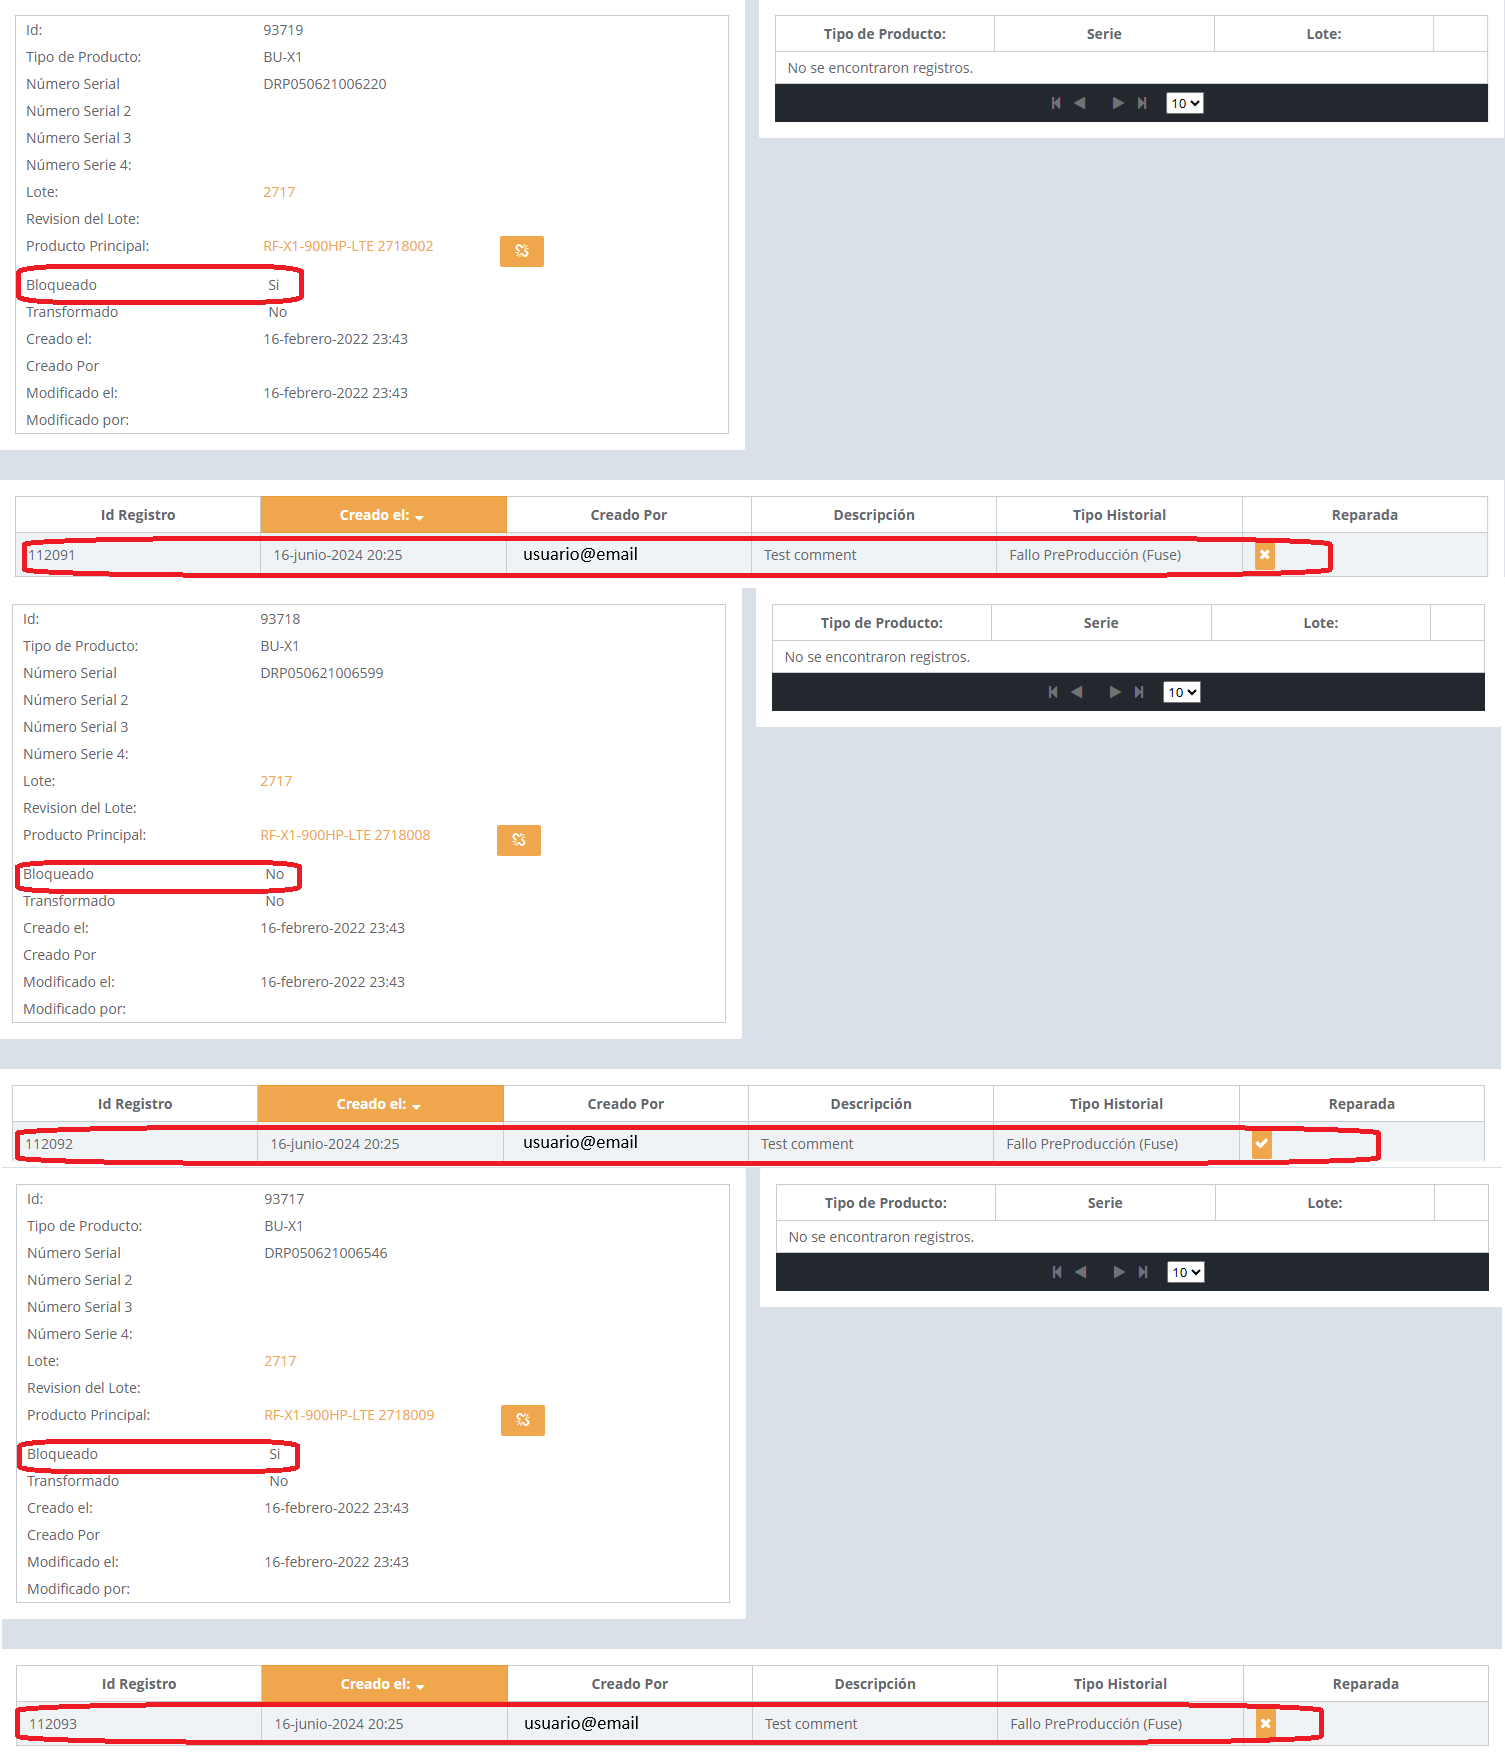
\includegraphics[width=1\textwidth]{validation-op-cm/test-1-products.png}
	\caption{\label{fig:op-test-1-products-cm} Comentario Múltiple: Productos después del registro de historias.}
\end{figure}

\subsection{DROPCONTROL}

\subsubsection{FÓRMULAS}

Primero se debe acceder a la herramienta de \textbf{Dashboard Libre} en el menú del nuevo \textbf{DropControl} como muestra en en la figura \ref{fig:dash-libre-menu}.

\begin{figure}[H]
	\centering
	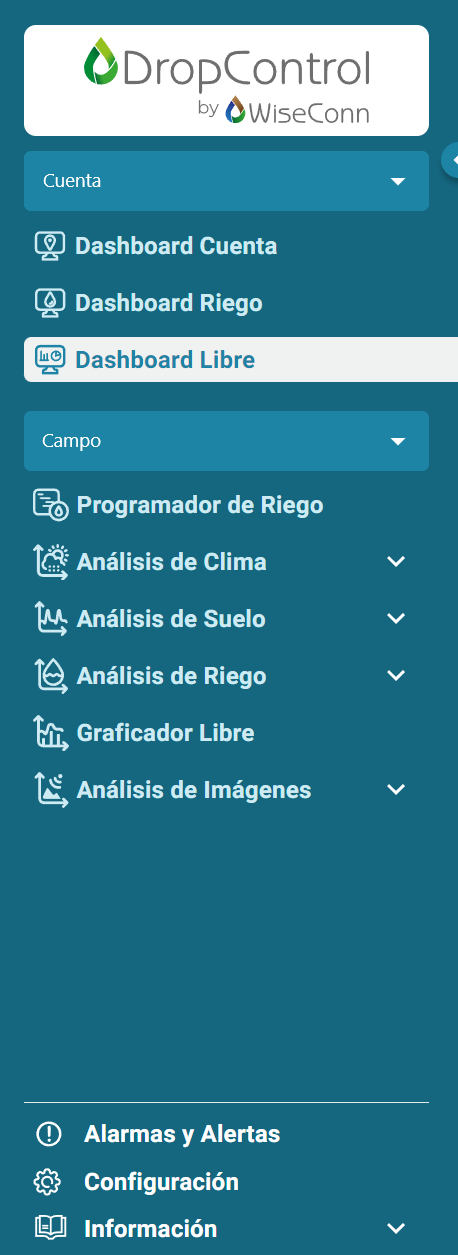
\includegraphics[width=1\textwidth]{widget-formulas/dashboard-libre-menu}
	\caption{\label{fig:dash-libre-menu} \textbf{Dashboard Libre} en el nuevo \textbf{DropControl}. Fuente: Elaboración propia.}
\end{figure}

Seleccionar o crear un \textit{dashboard}. Entrar al modo edición en la esquina superior derecha como muestra en la figura \ref{fig:entrar-modo-edicion}.
\iffalse foto con paso de como entrar al modo edicion \fi
\begin{figure}[H]
	\centering
	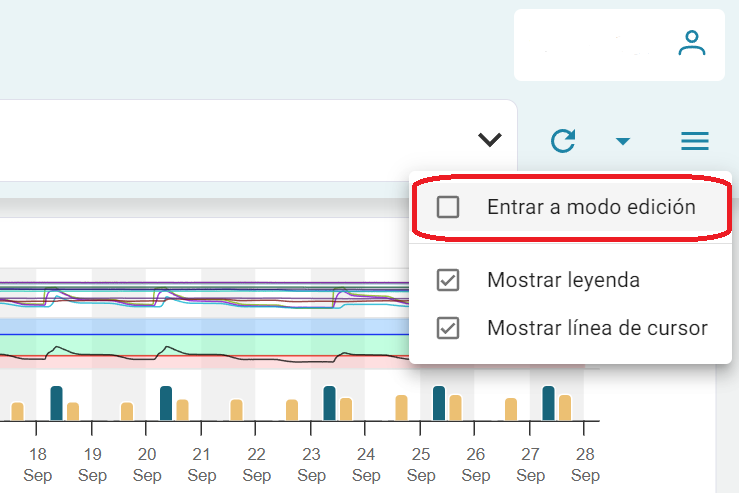
\includegraphics[width=1\textwidth]{widget-formulas/entrar-modo-edicion.png}
	\caption{\label{fig:entrar-modo-edicion} Entrar a modo edición. Elaboración propia.}
\end{figure}

Al estar en modo edición, para acceder a los formularios de \textit{widget} de tabla y/o gráfico existen 2 opciones:
\begin{itemize}
	\item Crear un nuevo \textit{widget} haciendo clic en el botón 'Crear...' en la esquina superior derecha (figura \ref{fig:opciones-crear}).
	\item Editar un \textit{widget} existente haciendo clic en el ícono de lápiz en la parte superior del \textit{widget} (figura \ref{fig:editar-widget}).
\end{itemize}
\iffalse pasos para ingresar al formulario de ambas formas \fi
\begin{figure}[H]
	\centering
	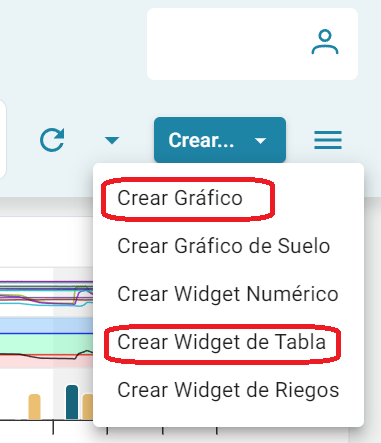
\includegraphics[width=1\textwidth]{widget-formulas/opciones-crear.png}
	\caption{\label{fig:opciones-crear} Crear \textit{widget} nuevo. Elaboración propia.}
\end{figure}
\begin{figure}[H]
	\centering
	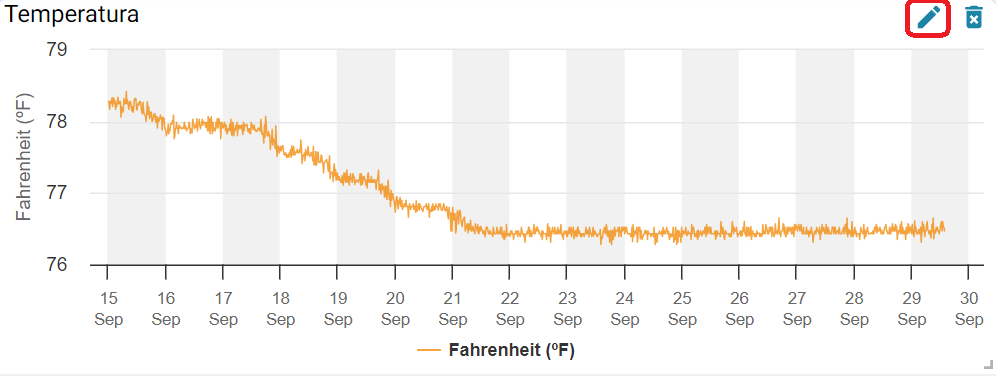
\includegraphics[width=1\textwidth]{widget-formulas/editar-widget.png}
	\caption{\label{fig:editar-widget} Editar \textit{widget} existente. Elaboración propia.}
\end{figure}

Se utilizará el formulario de gráfico para el paso a paso. Para este caso tenemos una variable de temperatura en unidad \textit{Fahrenheit} el cual vamos a convertir a \textit{Celsius}.
Al entrar al formulario del \textit{widget} entramos a la pestaña de fórmulas (figura \ref{fig:pestana-formulas}).
\iffalse ingresar a formulas \fi
\begin{figure}[H]
	\centering
	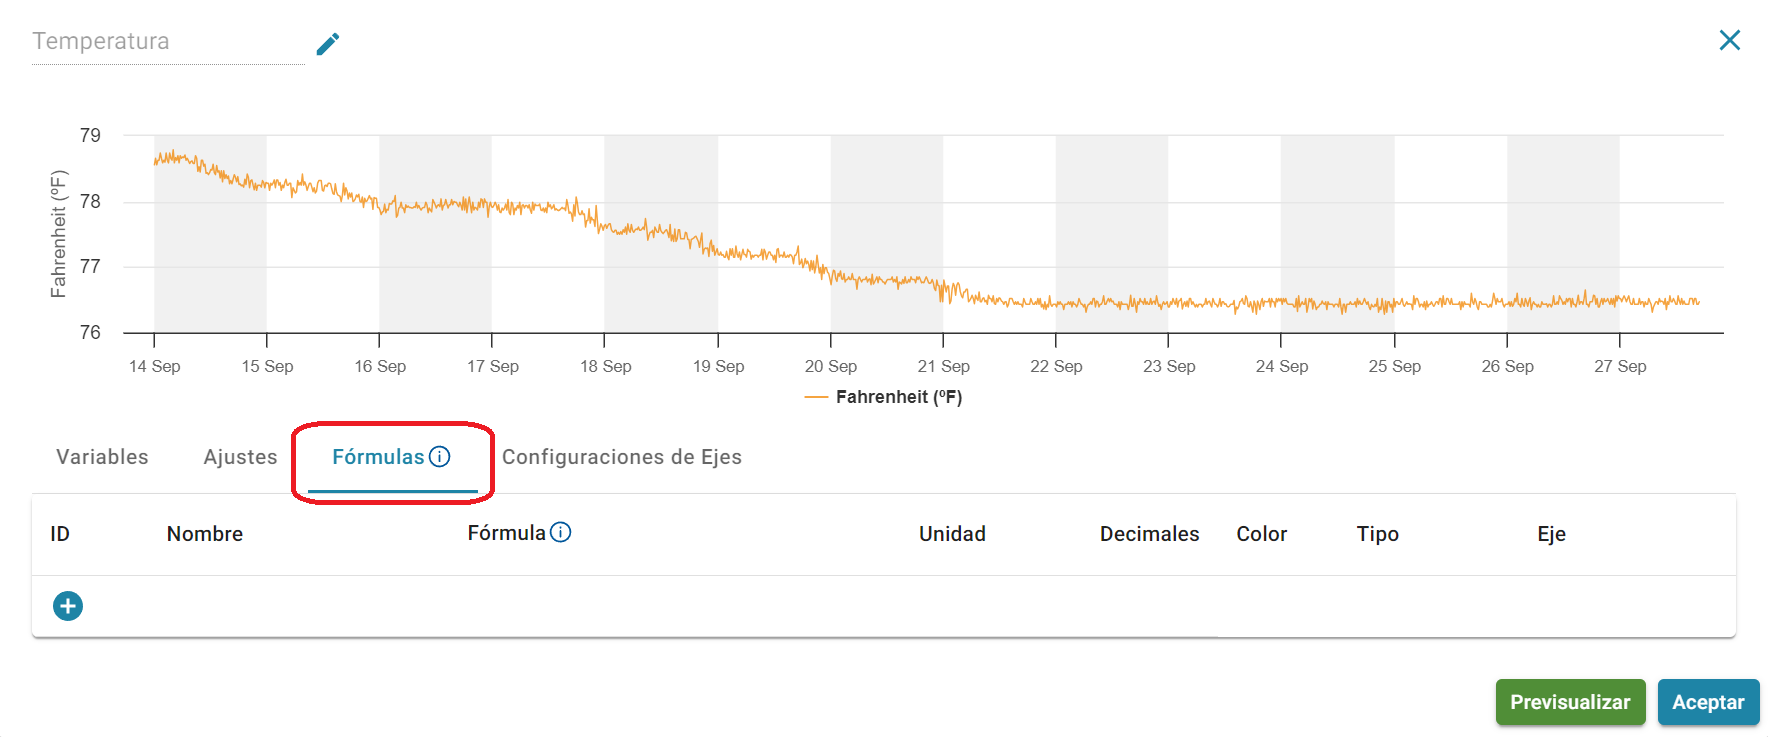
\includegraphics[width=1\textwidth]{widget-formulas/pestana-formulas.png}
	\caption{\label{fig:pestana-formulas} Editar \textit{widget} existente. Elaboración propia.}
\end{figure}
Primero rellenamos y seleccionamos todos los \textit{inputs} y dejamos el \textit{input} de fórmula para el final. Como muestra la figura \ref{fig:primer-relleno-formula}, la fórmula tendrá:
\begin{itemize}
	\item Nombre: \textbf{\textit{Celsius}}.
	\item Unidad: ºC
	\item \# Decimales: 3.
	\item Color: Rojo
	\item Tipo: Línea.
	\item Posición de eje: Derecha.
\end{itemize}
\iffalse relleno de inputs \fi
\begin{figure}[H]
	\centering
	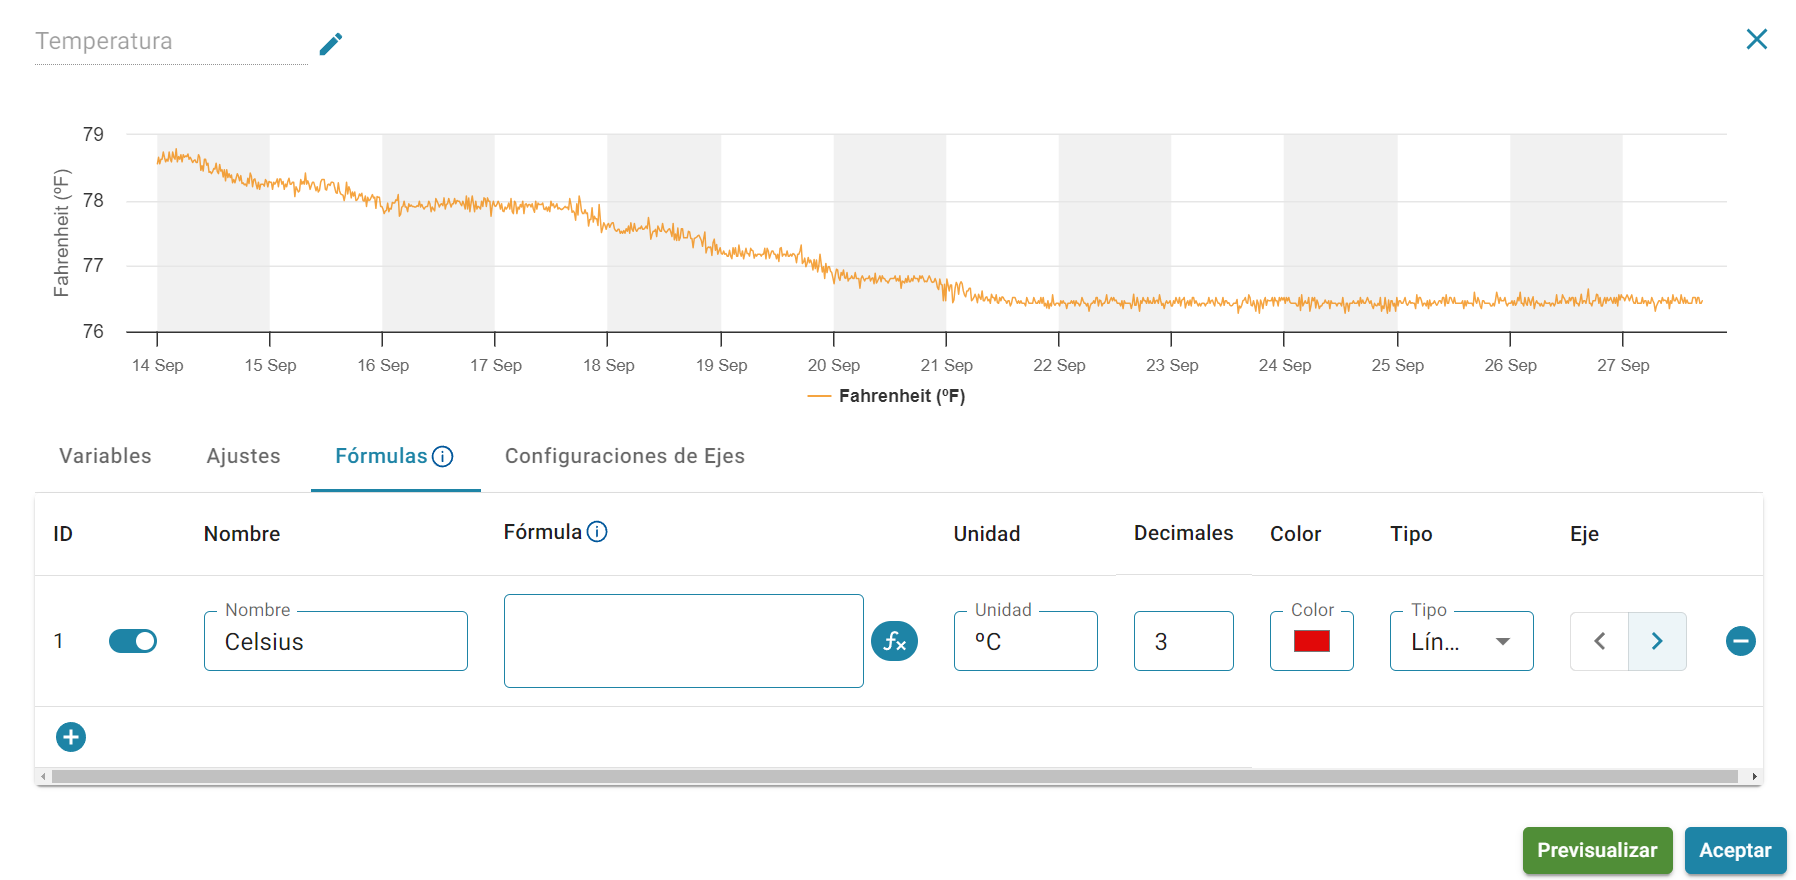
\includegraphics[width=1\textwidth]{widget-formulas/primer-relleno-formula.png}
	\caption{\label{fig:primer-relleno-formula} Relleno de \textit{inputs}. Elaboración propia.}
\end{figure}

Se puede ingresar la fórmula completamente a mano o con el botón al lado del \textit{input}. En la figura \ref{fig:lista-boton} muestra la lista al hacer clic en el botón a lado del \textit{input} de formula.
\iffalse lista de boton \fi
\begin{figure}[H]
	\centering
	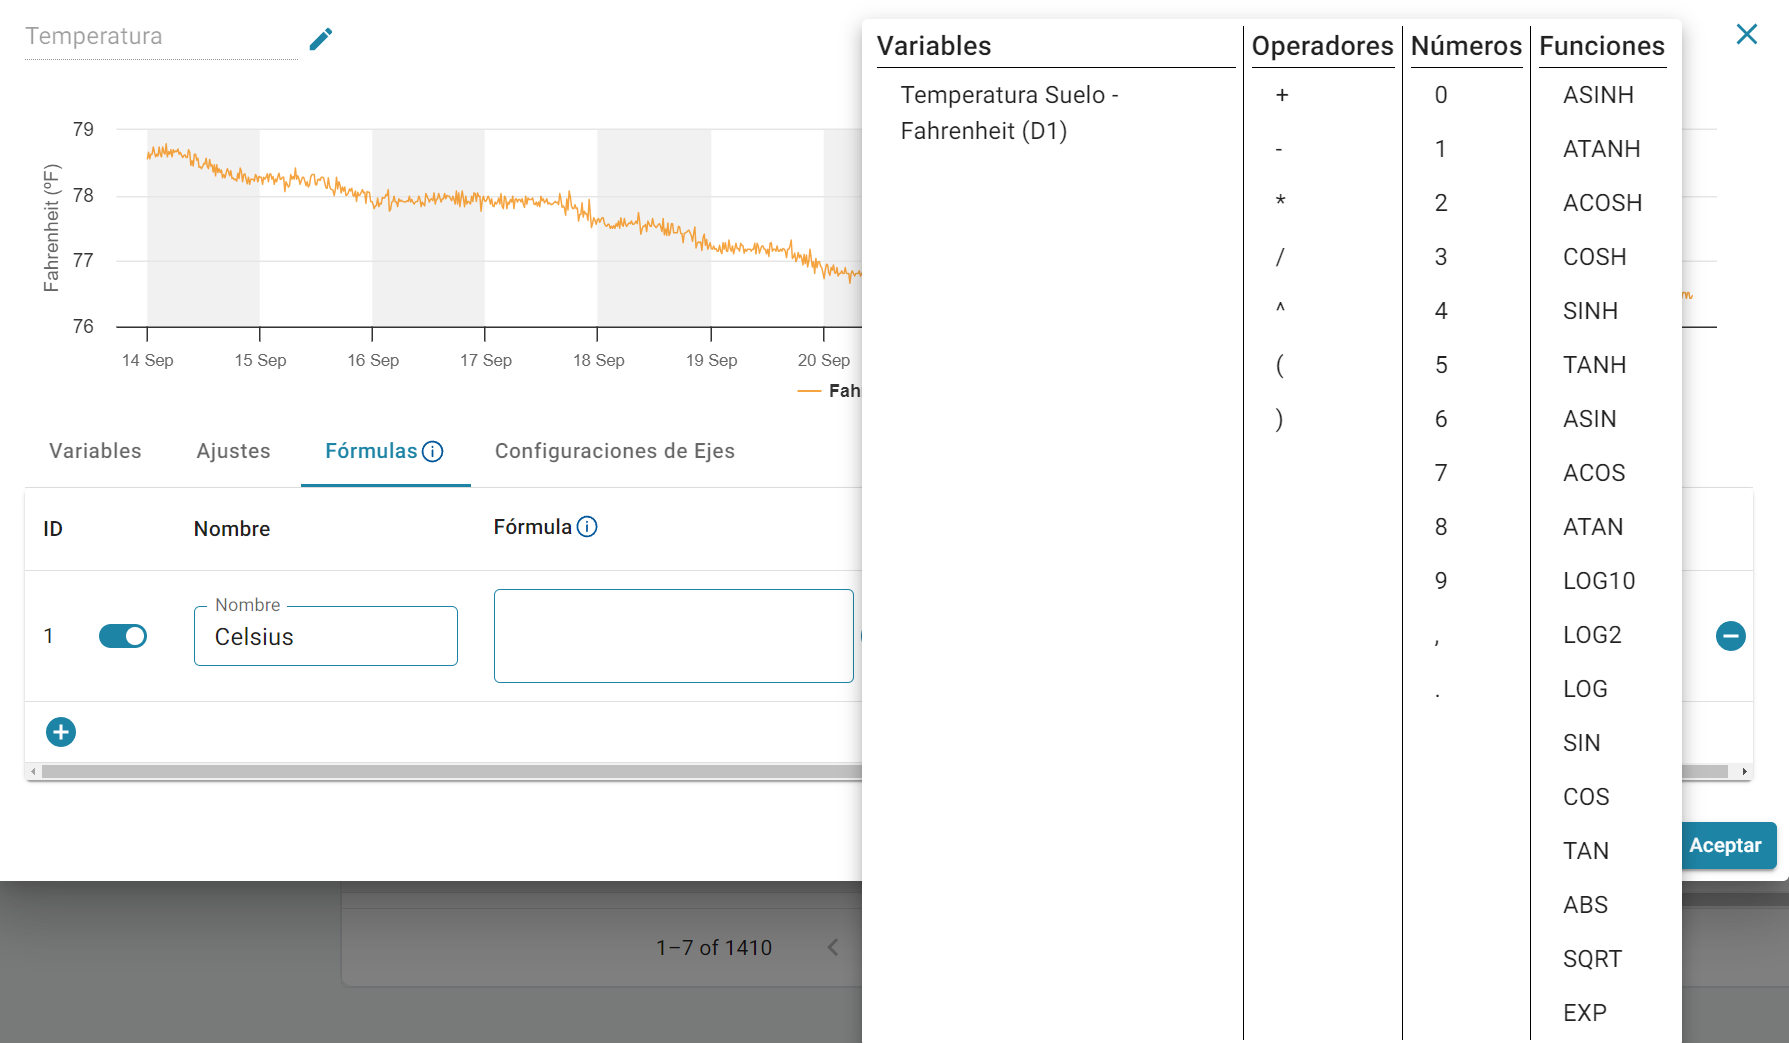
\includegraphics[width=1\textwidth]{widget-formulas/lista-boton.png}
	\caption{\label{fig:lista-boton} Lista al hacer clic en el botón a lado del \textit{input} de formula. Elaboración propia.}
\end{figure}

Se ingresa la fórmula para convertir desde \textit{Fahrenheit} a \textit{Celsius} (figura \ref{fig:formula-ingresada}).
\iffalse formula \fi
\begin{figure}[H]
	\centering
	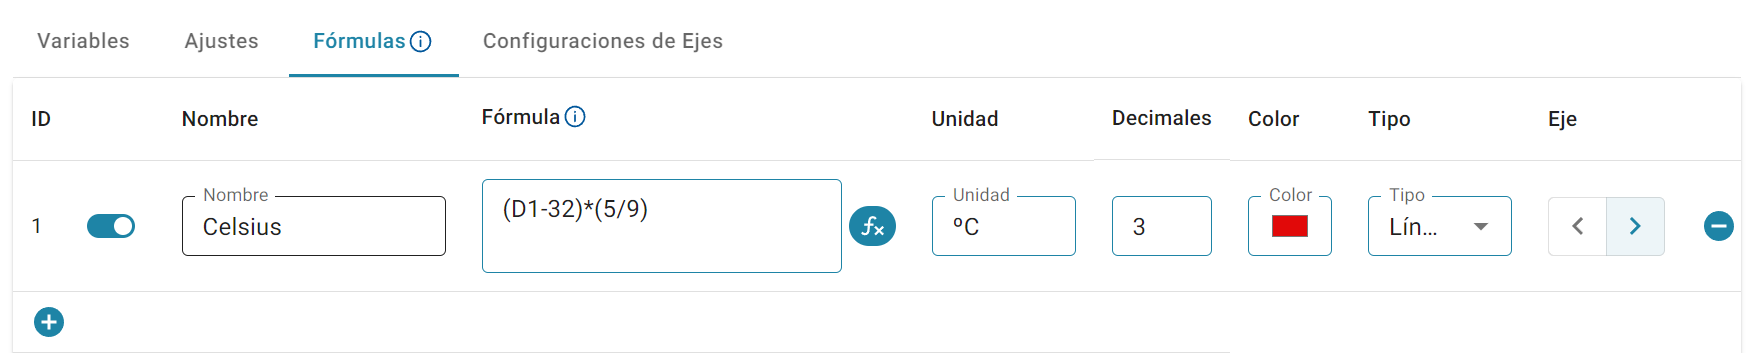
\includegraphics[width=1\textwidth]{widget-formulas/formula-ingresada.png}
	\caption{\label{fig:formula-ingresada} Formula de conversión de Fahrenheit a Celsius ingresada en el formulario. Elaboración propia.}
\end{figure}

Hacemos clic en el botón \textbf{Previsualizar}, esperamos a que muestre el gráfico en la parte superior del formulario, tomamos un punto como muestra en la figura \ref{fig:formula-preview} y comparamos un punto.
\iffalse formula previsualizada \fi
\iffalse formula con punto seleccionado \fi
\begin{figure}[H]
	\centering
	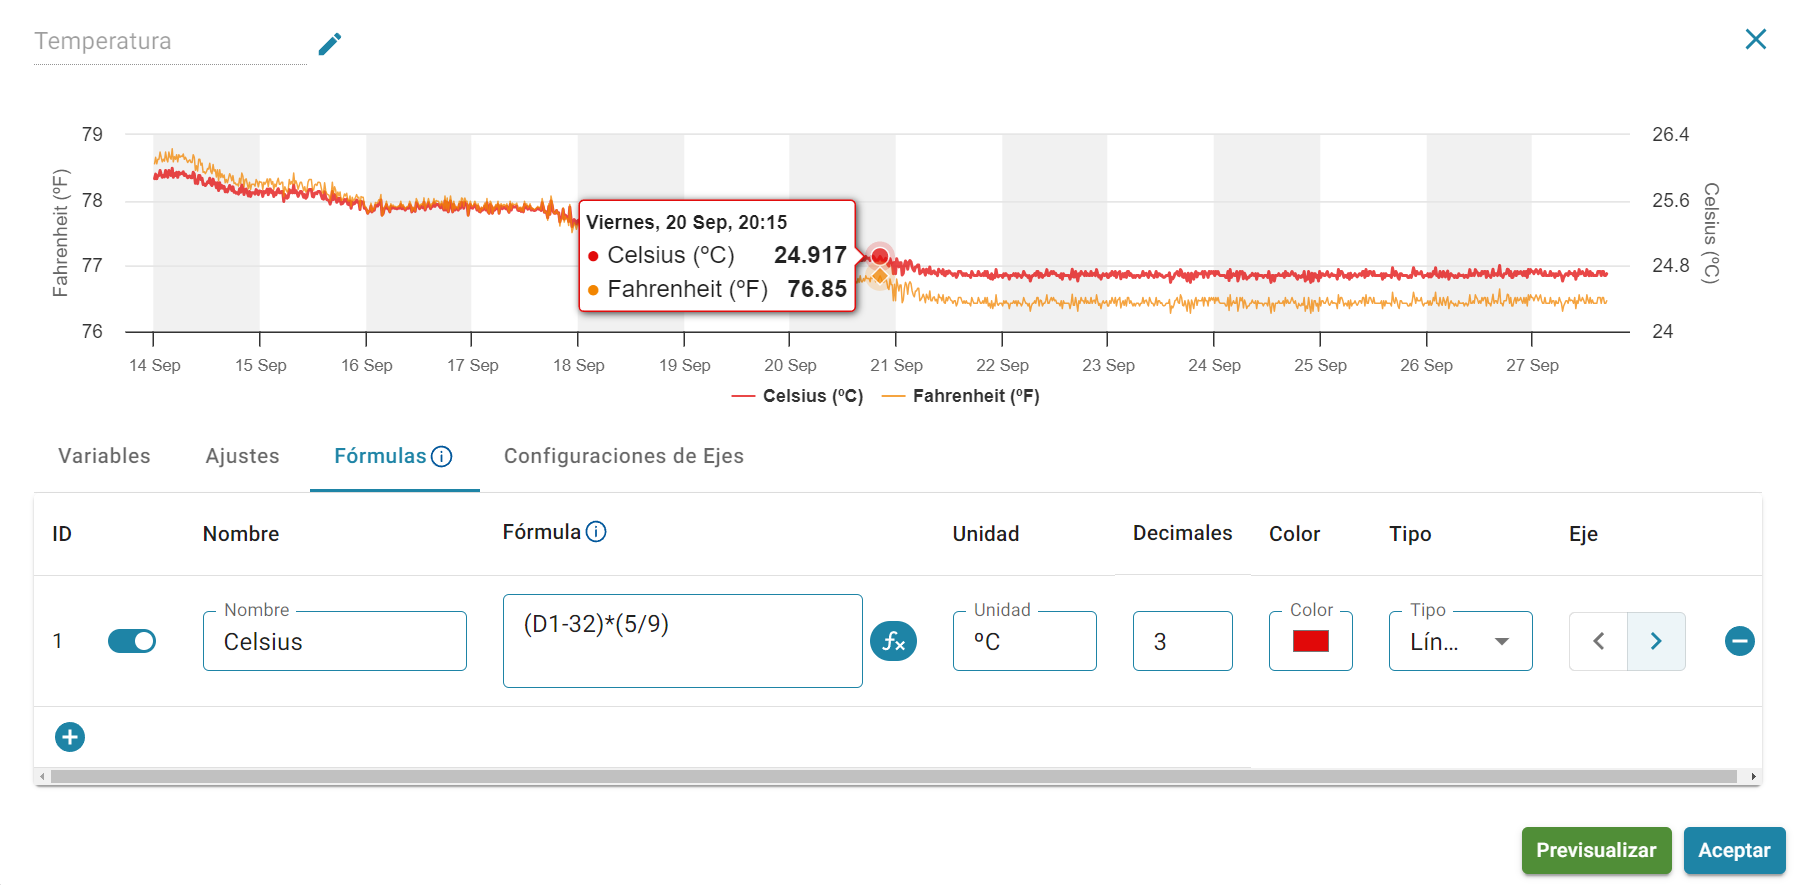
\includegraphics[width=1\textwidth]{widget-formulas/formula-preview.png}
	\caption{\label{fig:formula-preview} Previsualización de fórmula en el gráfico. Elaboración propia.}
\end{figure}

\iffalse agregar referencia a formulas \fi
Crearemos una segunda formula para una segunda variable de temperatura que convertiremos de Fahrenheit a Celsius como se muestra en la figura \ref{fig:dos-variables}. Luego, creamos una tercera fórmula con la suma de las fórmulas 1 y 2 (figura \ref{fig:suma-variables})
\begin{figure}[H]
	\centering
	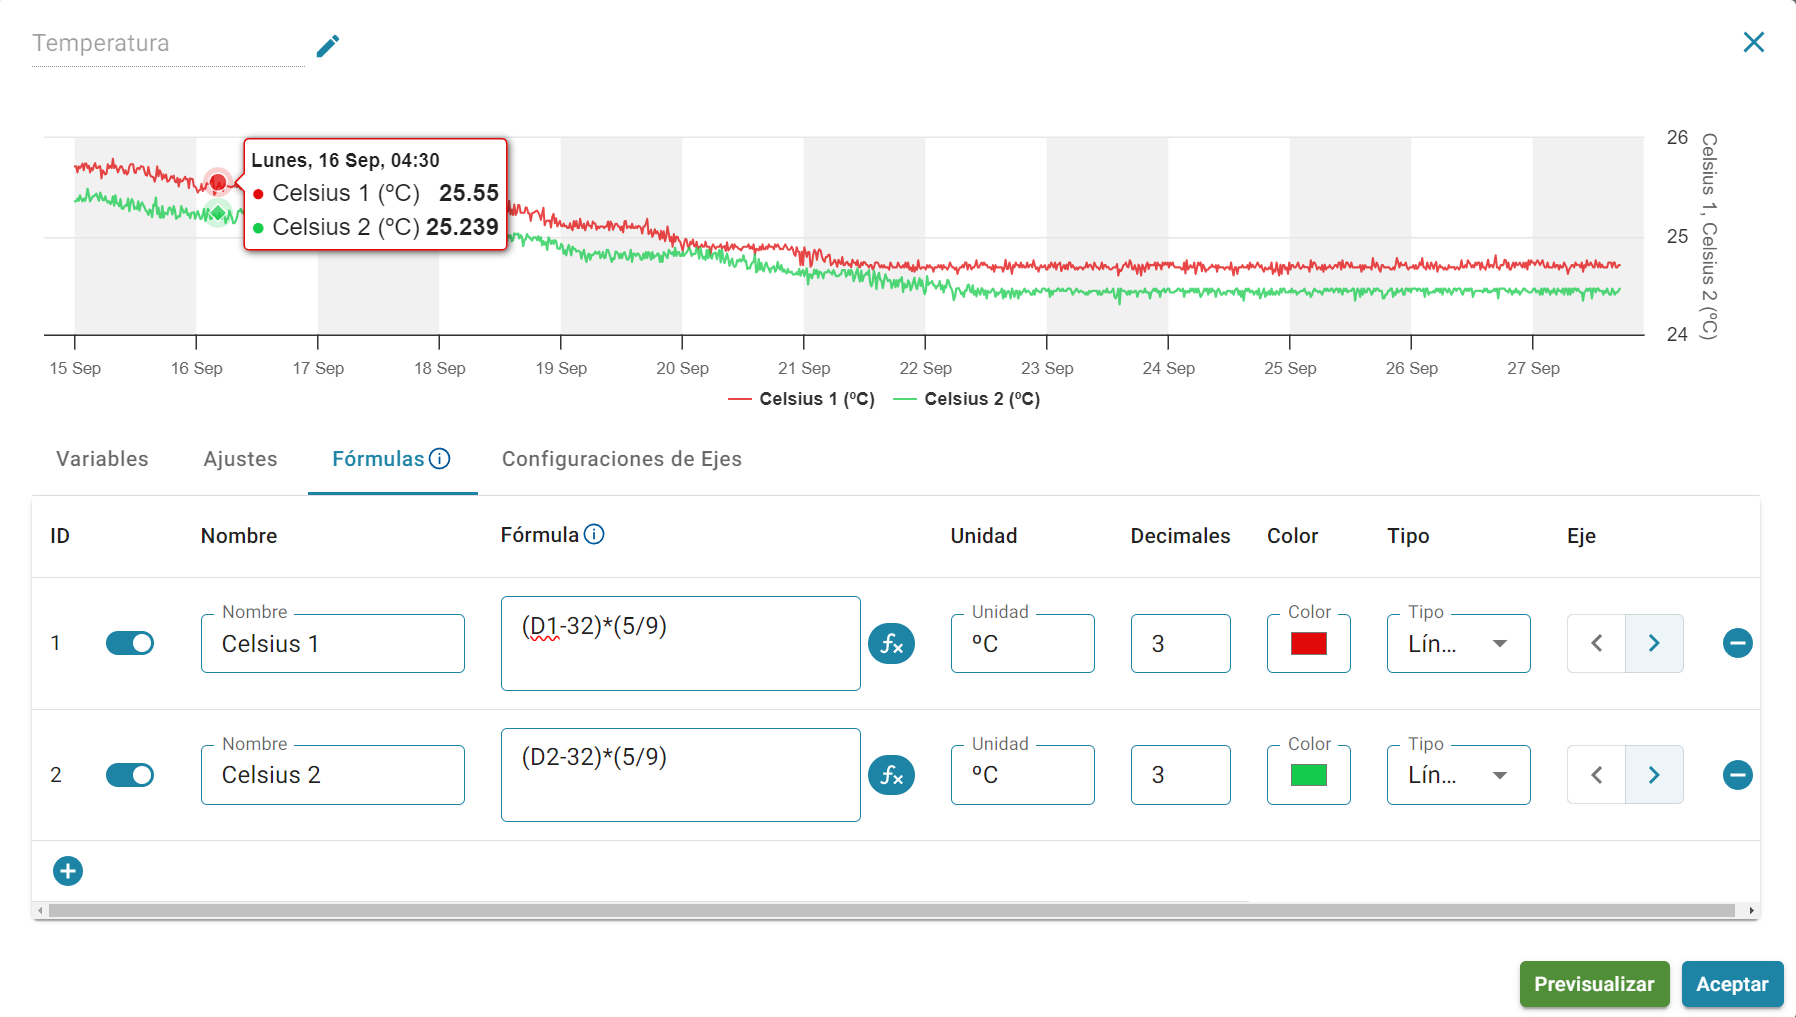
\includegraphics[width=1\textwidth]{widget-formulas/dos-variables.png}
	\caption{\label{fig:dos-variables} 2 conversiones de temperatura. Elaboración propia.}
\end{figure}

\begin{figure}[H]
	\centering
	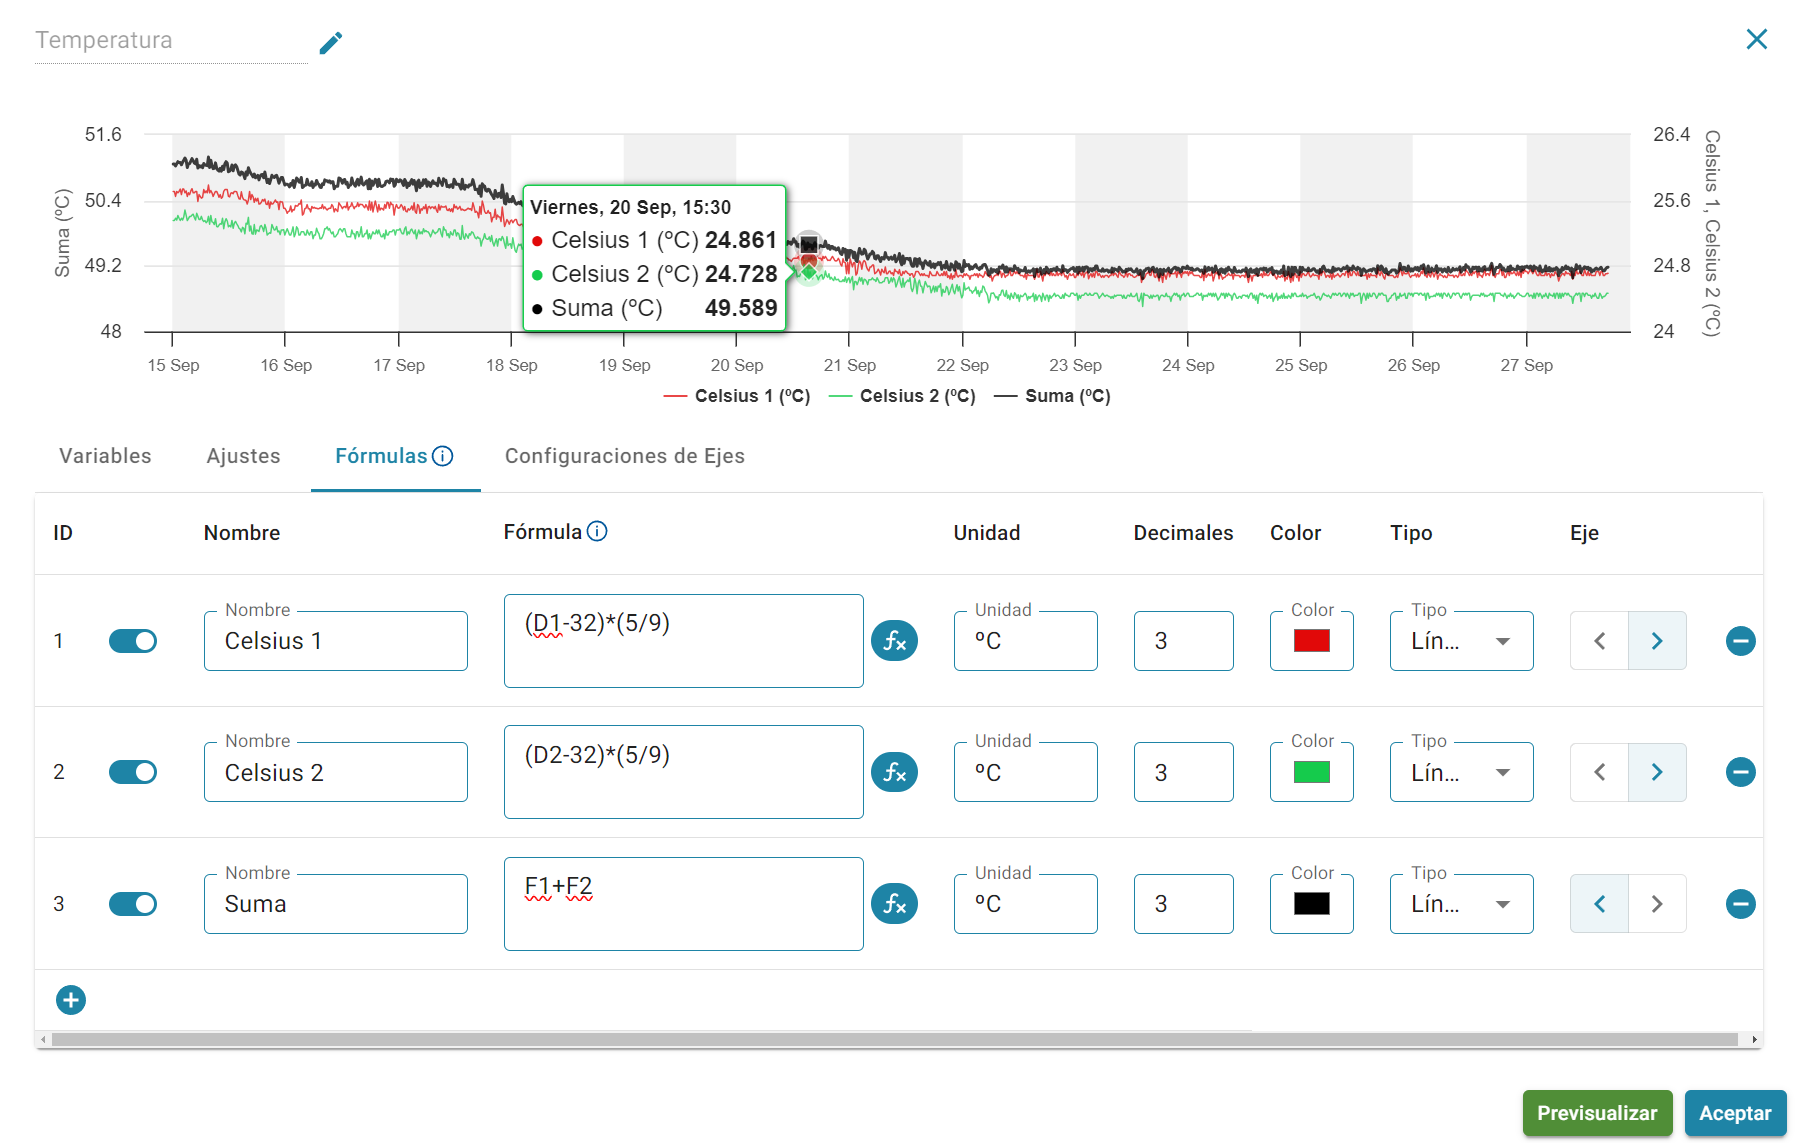
\includegraphics[width=1\textwidth]{widget-formulas/suma-variables.png}
	\caption{\label{fig:suma-variables} Referencia a fórmulas: Suma de 2 fórmulas. Elaboración propia.}
\end{figure}

Dentro de las validaciones del formularios están:
\begin{itemize}
    \item Debe contener solo caracteres válidos, es decir, la formula debe contener (figura ...): 
        \SubItem{Números. Si son números decimales se debe usar separador de decimales ya sea punto o coma. Los números no deben contener separados de miles.} 
        \SubItem{Operadores matemáticos: '+' (suma), '-' (resta), '*' (multiplicación), '/' (división) y '\^{}' (potencia).}
        \SubItem{Paréntesis.}
        \SubItem{Funciones soportadas.}
    \item La fórmula debe tener al menos una variable o referencia a una fórmula (figura ...).
    \item No pueden existir referencias circulares al hacer referencias a otras fórmulas (figura ...).
    \item Las variables y fórmulas referenciadas en la fórmula deben existir en el \textit{widget} (figura ...).        
\end{itemize}
\iffalse
\subsection{SETUP}

\subsubsection{CONFIGURADOR DE FUENTES}

En el configurador \textit{Wizard} de \textit{Setup}, al llegar al paso 'Opciones' se encuentran distintas configuraciones que se pueden realizar, dentro de estas se encuentra 'Configuración de Fuentas' como muestra en la figura \ref{fig:ws-wizard-option}

\begin{figure}[H]
	\centering
	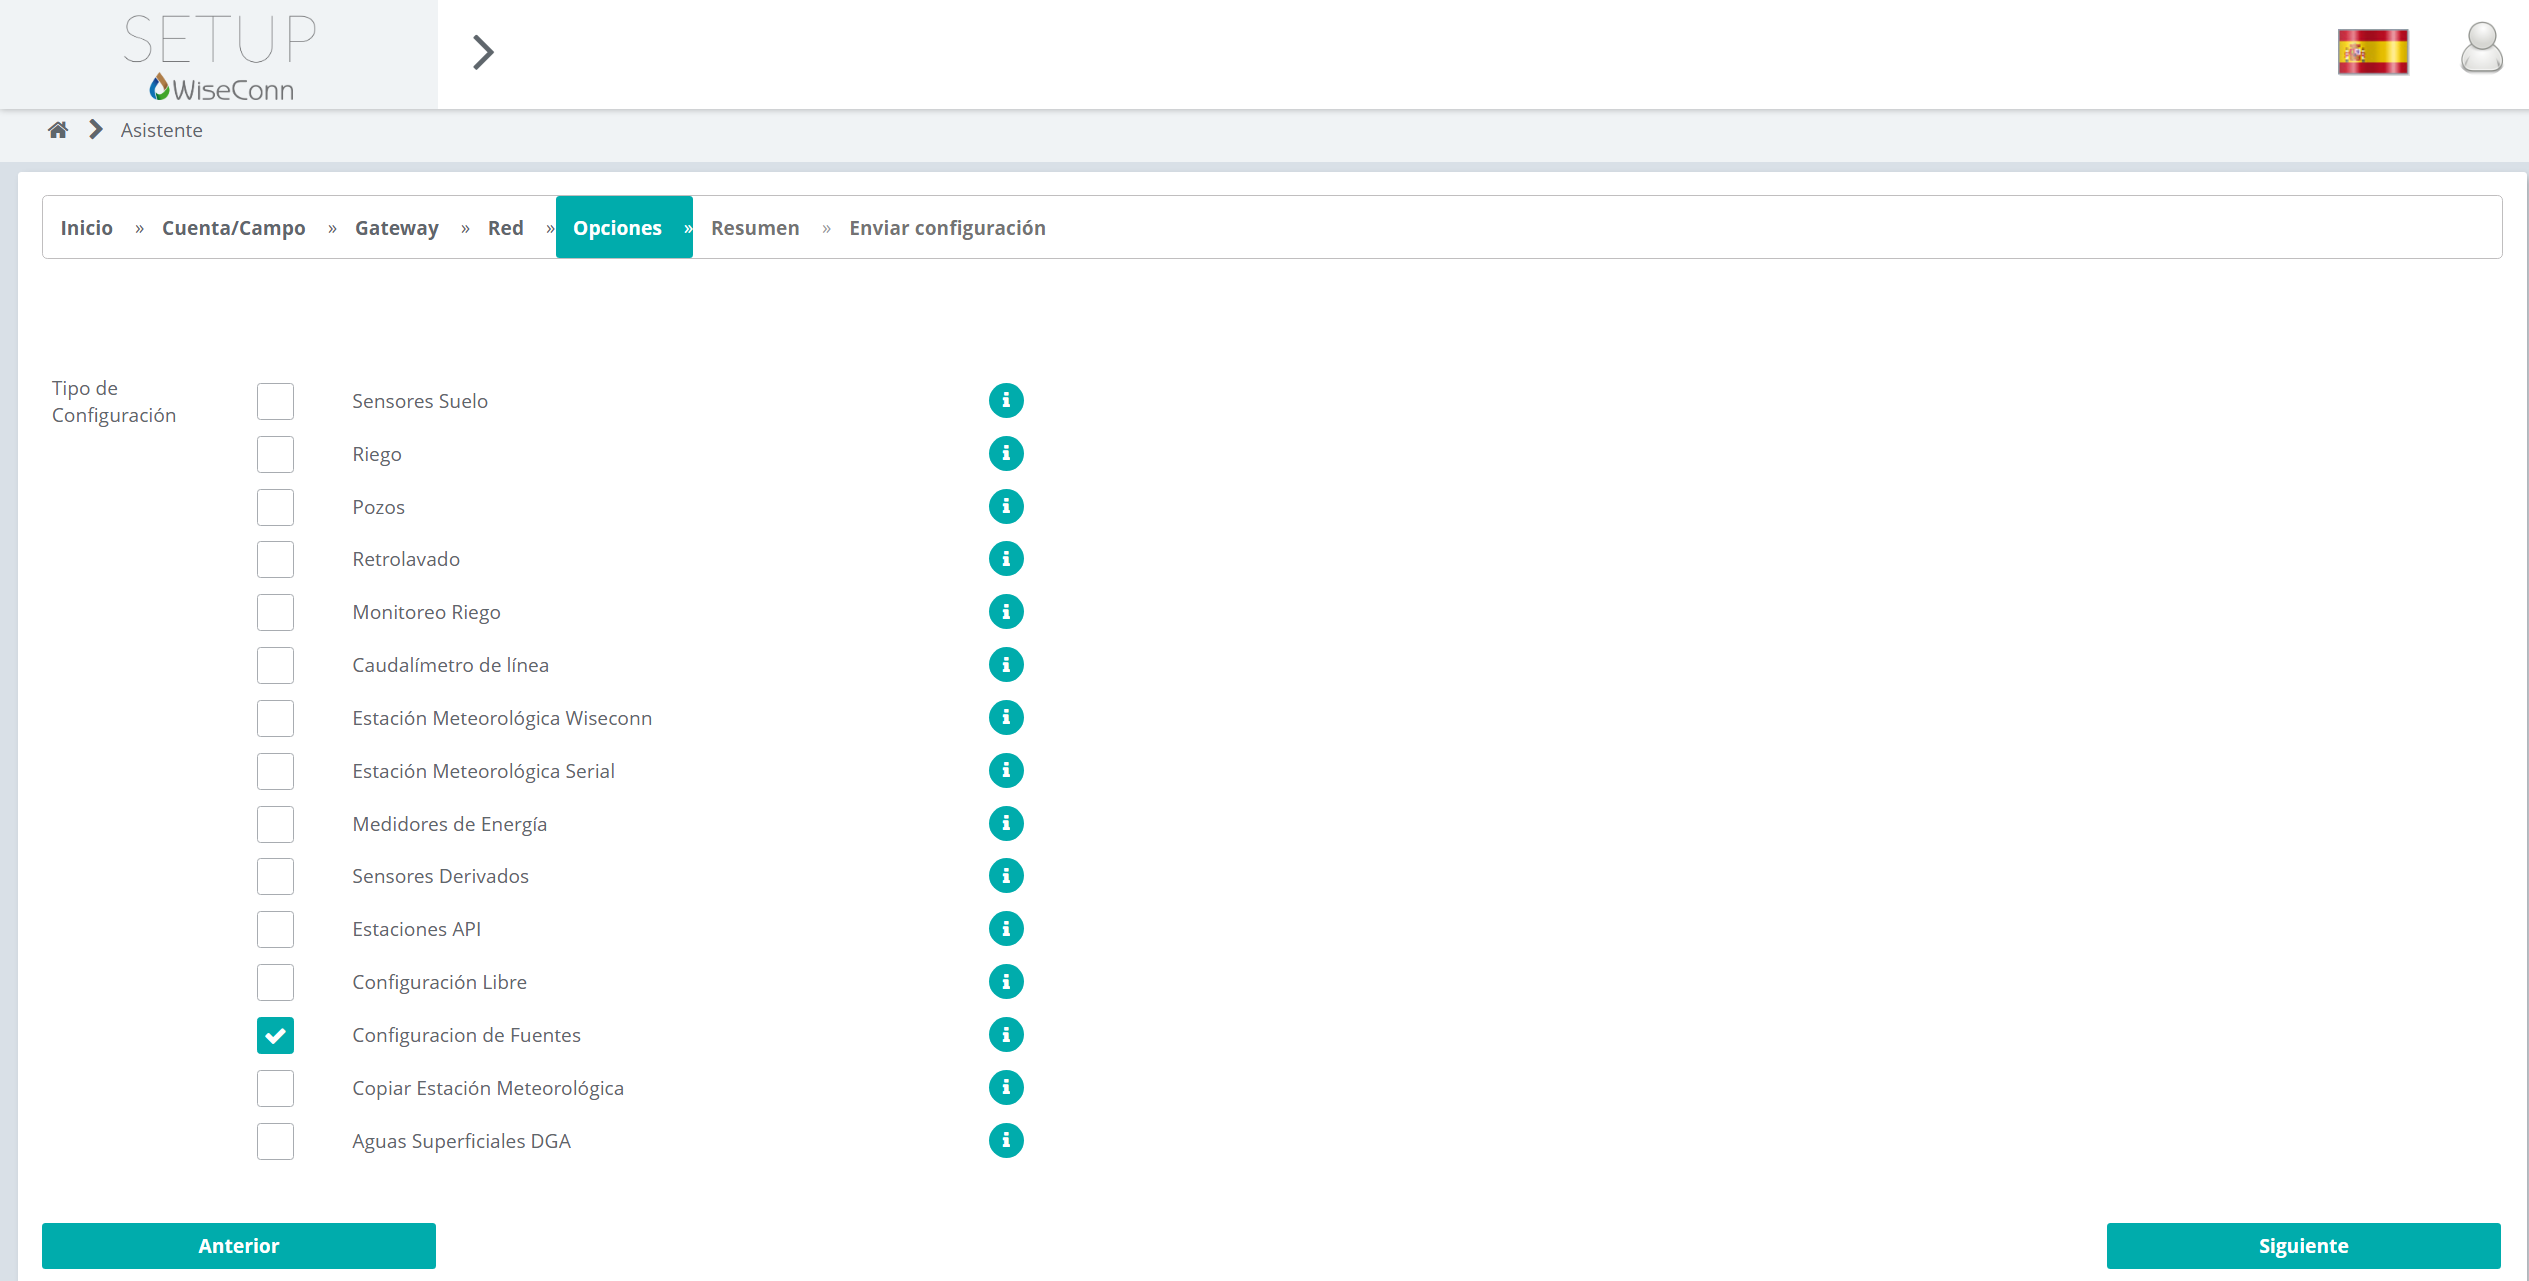
\includegraphics[width=1\textwidth]{validation-watersources/wizard-option.png}
	\caption{\label{fig:ws-wizard-option} Configuración de Fuentes en el asistente de configuración \textit{Wizard}}
\end{figure}

Al seleccionar la opción de 'Configuración de Fuentes' y hacer click en siguiente, se redirige a la herramienta.

\begin{figure}[H]
	\centering
	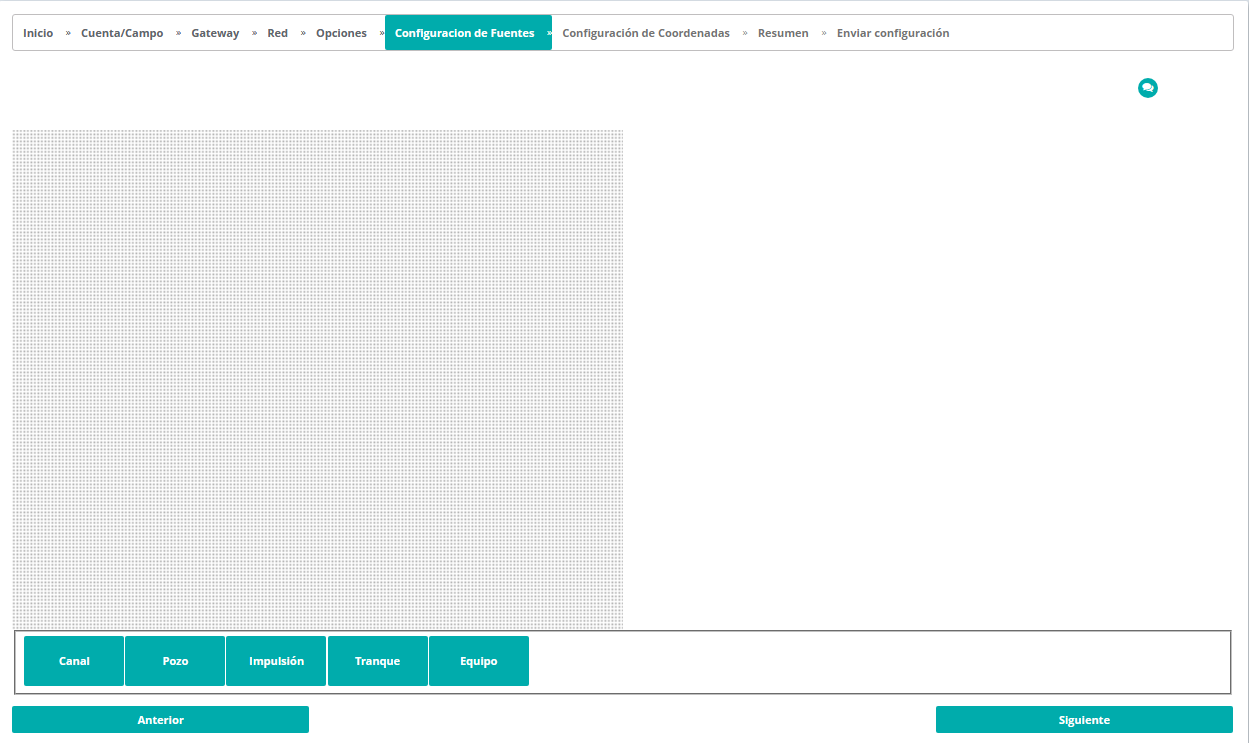
\includegraphics[width=0.8\textwidth]{water-view}
	\caption{\label{fig:water-view} Configurador de fuentes. Fuente: Elaboración propia.}
\end{figure}

A continuación se mostrarán las conexiones permitidas según muestra la figura \ref{fig:water-connections}:

\begin{figure}[H]
	\centering
	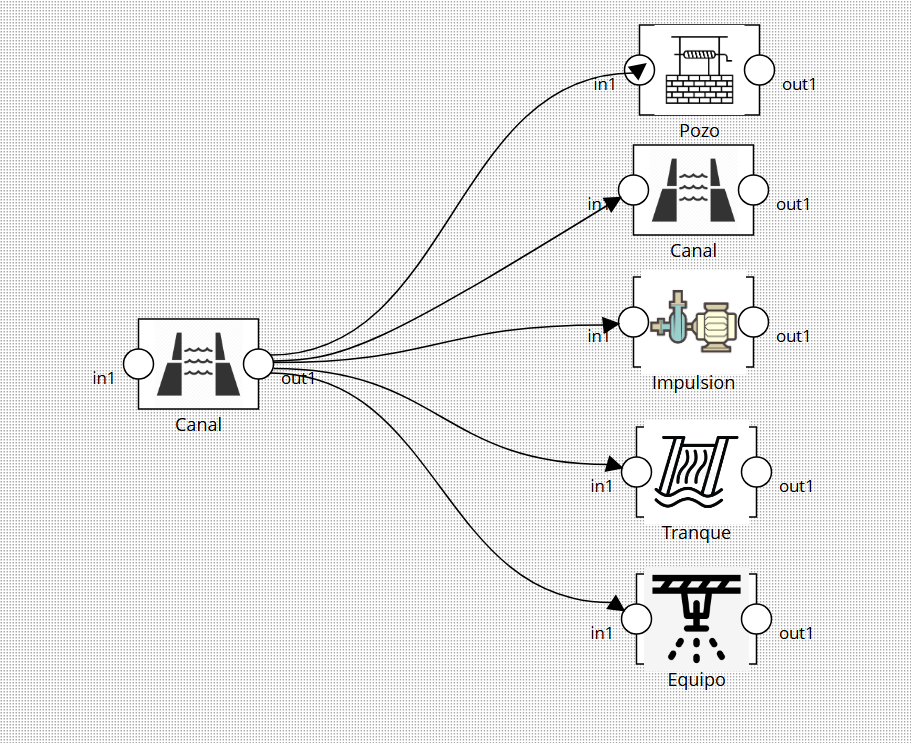
\includegraphics[width=0.8\textwidth]{validation-watersources/from-canal.png}
	\caption{\label{fig:from-canal} Conexiones desde un canal. Fuente: Elaboración propia.}
\end{figure}

\begin{figure}[H]
	\centering
	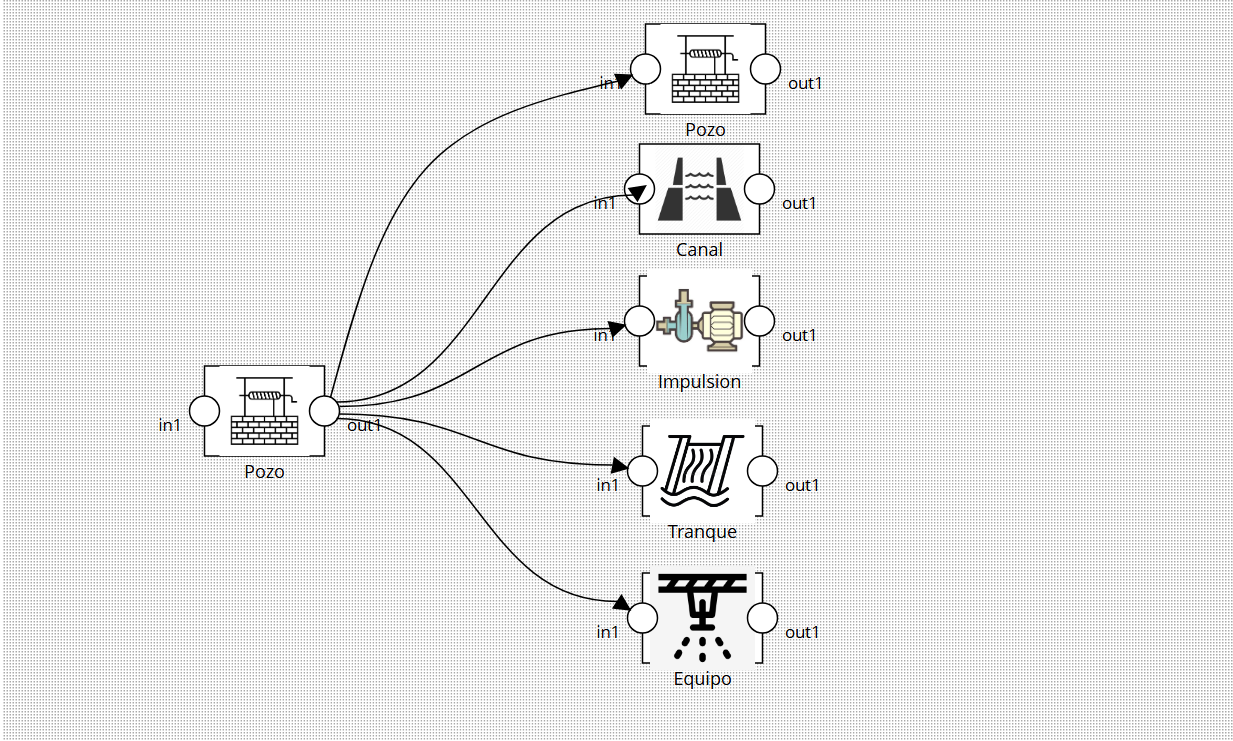
\includegraphics[width=0.8\textwidth]{validation-watersources/from-pozo.png}
	\caption{\label{fig:from-pozo} Conexiones desde un pozo. Fuente: Elaboración propia.}
\end{figure}

\begin{figure}[H]
	\centering
	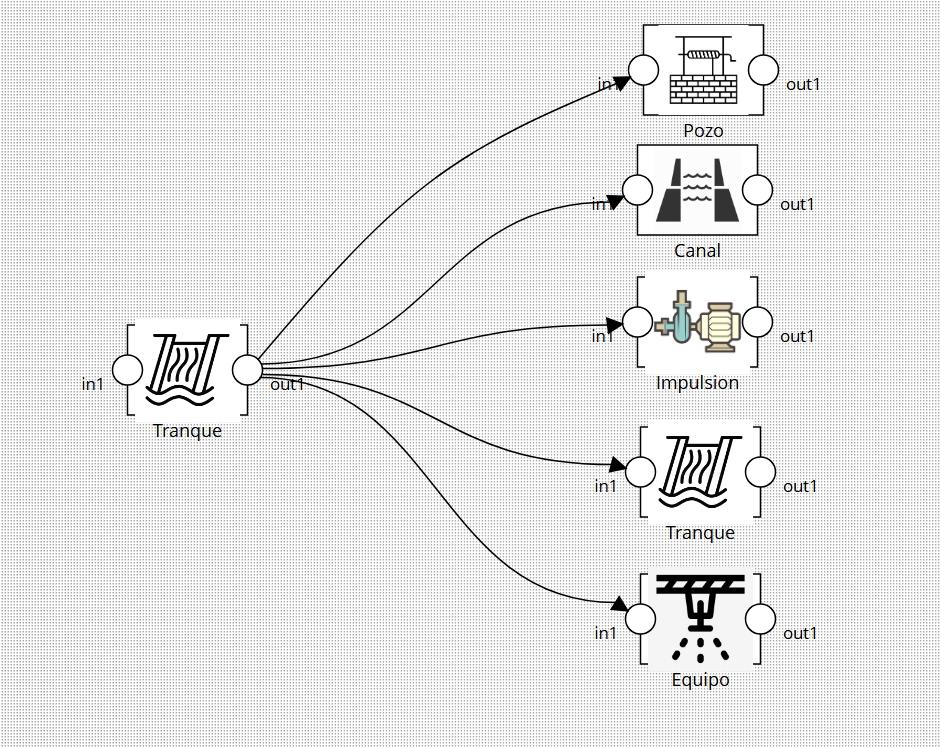
\includegraphics[width=0.8\textwidth]{validation-watersources/from-tranque.png}
	\caption{\label{fig:from-tranque} Conexiones desde un tranque. Fuente: Elaboración propia.}
\end{figure}

\begin{figure}[H]
	\centering
	\includegraphics[width=0.8\textwidth]{validation-watersources/from-impulsion.png}
	\caption{\label{fig:from-impulsion} Conexiones desde una impulsión. Fuente: Elaboración propia.}
\end{figure}

\begin{figure}[H]
	\centering
	\includegraphics[width=0.8\textwidth]{validation-watersources/from-equipo.png}
	\caption{\label{fig:from-equipo} Conexiones desde un equipo de riego. Fuente: Elaboración propia.}
\end{figure}
\fi